\documentclass[11pt, a4paper, oneside]{article}

% Originally developed by Andreas Wieser and Prof. Manfred Einsiedler.

% \documentclass[11pt,a4paper,oneside]{book}

% Default packages and configurations {{{
%%%%%%%%%%%%%%%%%%%%%%%%%%%%%%%%%%%%%%%%%%%%%%%%%%%%%%%%%%%%%%%%%%%%%%%%%%%%%%%%

\usepackage[T1]{fontenc}
\usepackage{amscd}
\usepackage{amsfonts}
\usepackage{amsmath}
\usepackage{amssymb}
\usepackage{amsthm}
% \usepackage{comment}
\usepackage{dsfont}
\usepackage{enumerate}
% \usepackage{faktor}
\usepackage{fancyhdr}


%% STUART BIB URL BREAK
\usepackage{url}
\def\UrlBreaks{\do\/\do-}


\usepackage[hidelinks]{hyperref}
% Colour settings for hyperlink references
% \hypersetup{%
%   colorlinks=false,
%   allcolors=black,
%   pdfborderstyle={/S/U/W 1} % Underline of width 1pt
% }
\hypersetup{%
  colorlinks,
  allcolors=black
}
\usepackage[nameinlink]{cleveref}

\usepackage{indentfirst}
% \usepackage{mathtools}
% \usepackage{url}
\usepackage{verbatim}
% \usepackage{xspace}

% Figures
\usepackage[final]{graphicx}
% \usepackage{caption}
\usepackage{float}
% \usepackage{import}
% \usepackage{pdfpages}
% \usepackage{subcaption}
% Note, graphicx must be imported before tikz
\usepackage{tikz-cd}
\usepackage{tikz}
% @legacy, used to have 'quotes' tikzlibrary as well
\usetikzlibrary{angles,arrows,calc,decorations.pathmorphing,matrix,shapes}
% \usepackage{transparent}
% \usepackage{xifthen}

% }}} %%%%%%%%%%%%%%%%%%%%%%%%%%%%%%%%%%%%%%%%%%%%%%%%%%%%%%%%%%%%%%%%%%%%%%%%%%
% Page Layout {{{
%%%%%%%%%%%%%%%%%%%%%%%%%%%%%%%%%%%%%%%%%%%%%%%%%%%%%%%%%%%%%%%%%%%%%%%%%%%%%%%%
% Setting white space {{{
%%%%%%%%%%%%%%%%%%%%%%%%%%%%%%%%%%%%%%%%%%%%%%%%%%%%%%%%%%%%%%%%%%%%%%%%%%%%%%%%

\usepackage{vmargin}
\RequirePackage[ansinew]{inputenc}
% {L}{T}{R}{B}{Head height}{Head separation}{Foot height}{Foot separation}
\setmarginsrb{1.25in}{0.6in}{1.25in}{0.8in}{20pt}{0.25in}{9pt}{0.3in}

% Set line spacing to 1.25
\usepackage{setspace}
\setstretch{1.2}
\setlength{\parskip}{0.25em}

% Kill indent at first line of new paragraphs
\setlength{\parindent}{15pt}

% Let height of page content vary from page to page (instead of stretching text
% body)
\raggedbottom

% Manage justification rules
\doublehyphendemerits=10000    % No consecutive line hyphens.
\brokenpenalty=10000           % No broken words across columns/pages.
\widowpenalty=9999             % Almost no widows at bottom of page.
\clubpenalty=9999              % Almost no orphans at top of page.
\interfootnotelinepenalty=9999 % Almost never break footnotes.
\binoppenalty=9999             % Almost never break binary operators.
\relpenalty=9999               % Almost never break binary relations.

% }}} %%%%%%%%%%%%%%%%%%%%%%%%%%%%%%%%%%%%%%%%%%%%%%%%%%%%%%%%%%%%%%%%%%%%%%%%%%
% Headers and footers {{{
%%%%%%%%%%%%%%%%%%%%%%%%%%%%%%%%%%%%%%%%%%%%%%%%%%%%%%%%%%%%%%%%%%%%%%%%%%%%%%%%

% Fancy has a header- and footer-rule, see below
\pagestyle{fancy}
% Clear old settings for headers and footers
\fancyhf{}

% Only mark the name of section
% N.b: This will be the last section starting on current page
\renewcommand{\sectionmark}[1]{\markright{#1}}

% Set line width for header and footer
\renewcommand{\headrulewidth}{0.6pt}
\renewcommand{\footrulewidth}{0.6pt}

% Clear old settings
\lhead{}
\rhead{}
\rfoot{\thepage}
\lfoot{}

% Use same settings as prescribed in default pagestyle

\fancypagestyle{plain}{%
  \fancyhf{}                           % Clear old settings
  \fancyfoot[R]{\thepage}              % ...except the right footer
  \renewcommand{\headrulewidth}{0.6pt} % Set line strength for header
  \renewcommand{\footrulewidth}{0.6pt} % Set line strength for footer
}

% Using this for title page
\newcommand{\HRule}{\rule{\linewidth}{0.5mm}}
% }}} %%%%%%%%%%%%%%%%%%%%%%%%%%%%%%%%%%%%%%%%%%%%%%%%%%%%%%%%%%%%%%%%%%%%%%%%%%
% Miscellaneous
%%%%%%%%%%%%%%%%%%%%%%%%%%%%%%%%%%%%%%%%%%%%%%%%%%%%%%%%%%%%%%%%%%%%%%%%%%%%%%%%

% Force footnotes to the bottom of the page
\usepackage[bottom]{footmisc}
% }}} %%%%%%%%%%%%%%%%%%%%%%%%%%%%%%%%%%%%%%%%%%%%%%%%%%%%%%%%%%%%%%%%%%%%%%%%%%
% Text Body {{{
%%%%%%%%%%%%%%%%%%%%%%%%%%%%%%%%%%%%%%%%%%%%%%%%%%%%%%%%%%%%%%%%%%%%%%%%%%%%%%%%
% Typesetting tools
%%%%%%%%%%%%%%%%%%%%%%%%%%%%%%%%%%%%%%%%%%%%%%%%%%%%%%%%%%%%%%%%%%%%%%%%%%%%%%%%

\newcounter{lecture}
\newcommand{\lecture}[1]{%
  \stepcounter{lecture}
  \marginpar{\color{orange}\flushleft{\footnotesize Lecture: \thelecture{} #1}}
}

\usepackage{mdframed}
\newmdenv[
  topline=false,
  bottomline=false,
  rightline=false,
  skipabove=\topsep,
  skipbelow=\topsep,
  innertopmargin=1pt,
  innerbottommargin=1pt,
  skipabove=10pt,
  skipbelow=10pt,
]{siderules}

% }}} %%%%%%%%%%%%%%%%%%%%%%%%%%%%%%%%%%%%%%%%%%%%%%%%%%%%%%%%%%%%%%%%%%%%%%%%%%
% Table of Contents {{{
%%%%%%%%%%%%%%%%%%%%%%%%%%%%%%%%%%%%%%%%%%%%%%%%%%%%%%%%%%%%%%%%%%%%%%%%%%%%%%%%

\usepackage{titlesec}
\usepackage[titles]{tocloft}
% Format section titles in TOC
\renewcommand\cftsecfont{\scshape}
% Format page numbers in TOC
\renewcommand\cftsecpagefont{\normalfont}
% @language Set name of TOC
\AtBeginDocument{\renewcommand\contentsname{Table of Contents}}

% }}} %%%%%%%%%%%%%%%%%%%%%%%%%%%%%%%%%%%%%%%%%%%%%%%%%%%%%%%%%%%%%%%%%%%%%%%%%%
% Bibliography {{{
%%%%%%%%%%%%%%%%%%%%%%%%%%%%%%%%%%%%%%%%%%%%%%%%%%%%%%%%%%%%%%%%%%%%%%%%%%%%%%%%

% Renew \cite command for more control of appearance
\let\defaultcite\cite
\renewcommand{\cite}[2][]{%
  \textnormal{\defaultcite[#1]{#2}}%
}

% }}} %%%%%%%%%%%%%%%%%%%%%%%%%%%%%%%%%%%%%%%%%%%%%%%%%%%%%%%%%%%%%%%%%%%%%%%%%%

% Generic tools {{{
%%%%%%%%%%%%%%%%%%%%%%%%%%%%%%%%%%%%%%%%%%%%%%%%%%%%%%%%%%%%%%%%%%%%%%%%%%%%%%%%

% When referencing lists, often we need two write things such as
% "\textit{(iii)}" which is long. This macro "enumerated reference" makes it
% easier.
% Usage: \eref{n}
\newcommand{\eref}[1]{\textit{(\romannumeral#1)}}

% }}} %%%%%%%%%%%%%%%%%%%%%%%%%%%%%%%%%%%%%%%%%%%%%%%%%%%%%%%%%%%%%%%%%%%%%%%%%%
% Math-Environments {{{
%%%%%%%%%%%%%%%%%%%%%%%%%%%%%%%%%%%%%%%%%%%%%%%%%%%%%%%%%%%%%%%%%%%%%%%%%%%%%%%%

% 1. \newtheorem{<Internal name>}{<External name>}[<env>]
%    Is counted after <env>. e.g.
%    \newtheorem{corollary}{Corollary}[theorem]
%    Theorem 1 is succeeded by Corollary 1.2
% 2. \newtheorem{<Internal name>}[<env>]{<External name>}[<env>]
%    \newtheorem{corollary}[theorem]{Corollary}
%    Is shares counter with <env>. i.e. Theorem 1 is succeeded by Corollary 2

% Declare a new theoremstyle
% \newtheoremstyle{mystyle}%
%    {3pt}                   % Space above
%    {3pt}                   % Space below
%    {\itshape\color{red}}   % Body font
%    {}                      % Indent amount
%    {\bfseries\color{blue}} % Theorem head font
%    {.}                     % Punctuation after theorem head
%    {.5em}                  % Space after theorem head
%    {}                      % Theorem head spec (can be left empty, meaning ‘normal’)

\theoremstyle{plain}

% Base number off chapter if documentclass 'book' is selected, else use
% sections.

\ifundef{\chapter}{%
  \newtheorem{theorem}{Theorem}[section]
  \numberwithin{equation}{section}
  \numberwithin{figure}{section}
}{%
  \newtheorem{theorem}{Theorem}[chapter]
  \numberwithin{equation}{chapter}
  \numberwithin{figure}{chapter}
}

\newtheorem*{theorem*}{Theorem}
\newtheorem{theorem-extra}{Theorem*}

\newtheorem{proposition}[theorem]{Proposition}
\newtheorem*{proposition*}{Proposition}
\newtheorem{proposition-extra}{Proposition*}

\newtheorem{lemma}[theorem]{Lemma}
\newtheorem*{lemma*}{Lemma}
\newtheorem{lemma-extra}{Lemma*}

\newtheorem*{fact}{Fact}

\newtheorem{corollary}[theorem]{Corollary}
\newtheorem*{corollary*}{Corollary}
\newtheorem{generic-corollary}[theorem]{Corollary}

\newtheorem{example}[theorem]{Example}
\newtheorem*{example*}{Example}

\newtheorem{exercise}[theorem]{Exercise}
\newtheorem*{exercise*}{Exercise}
\newtheorem{important-exercise}[theorem]{Important Exercise}

\newtheorem{reminder}[theorem]{Reminder}

\theoremstyle{remark}
  \newtheorem*{remark}{Remark}
\theoremstyle{plain}

\theoremstyle{definition}
  \newtheorem{definition}[theorem]{Definition}
  \newtheorem*{definition*}{Definition}
\theoremstyle{plain}

% }}} %%%%%%%%%%%%%%%%%%%%%%%%%%%%%%%%%%%%%%%%%%%%%%%%%%%%%%%%%%%%%%%%%%%%%%%%%%
% Mathematical notation
%%%%%%%%%%%%%%%%%%%%%%%%%%%%%%%%%%%%%%%%%%%%%%%%%%%%%%%%%%%%%%%%%%%%%%%%%%%%%%%%

% Tool for moving maths expressions
\makeatletter
\newcommand{\raisemath}[1]{\mathpalette{\raisemAth{#1}} }
\newcommand{\raisemAth}[3]{\raisebox{#1}{$#2#3$}}
\makeatother

\newcommand{\define}[1]{\textit{#1}}

% Special Letters {{{
%%%%%%%%%%%%%%%%%%%%%%%%%%%%%%%%%%%%%%%%%%%%%%%%%%%%%%%%%%%%%%%%%%%%%%%%%%%%%%%%

% For faster typesetting of the calligraphic letters
\newcommand{\bA}{\mathbb{A}}
\newcommand{\bB}{\mathbb{B}}
\newcommand{\bC}{\mathbb{C}}
\newcommand{\bD}{\mathbb{D}}
\newcommand{\bE}{\mathbb{E}}
\newcommand{\bF}{\mathbb{F}}
\newcommand{\bG}{\mathbb{G}}
\newcommand{\bH}{\mathbb{H}}
\newcommand{\bI}{\mathbb{I}}
\newcommand{\bJ}{\mathbb{J}}
\newcommand{\bK}{\mathbb{K}}
\newcommand{\bL}{\mathbb{L}}
\newcommand{\bM}{\mathbb{M}}
\newcommand{\bN}{\mathbb{N}}
\newcommand{\bO}{\mathbb{O}}
\newcommand{\bP}{\mathbb{P}}
\newcommand{\bQ}{\mathbb{Q}}
\newcommand{\bR}{\mathbb{R}}
\newcommand{\bS}{\mathbb{S}}
\newcommand{\bT}{\mathbb{T}}
\newcommand{\bU}{\mathbb{U}}
\newcommand{\bV}{\mathbb{V}}
\newcommand{\bW}{\mathbb{W}}
\newcommand{\bX}{\mathbb{X}}
\newcommand{\bY}{\mathbb{Y}}
\newcommand{\bZ}{\mathbb{Z}}

% For faster typesetting of the calligraphic letters
\newcommand{\cA}{\mathcal{A}}
\newcommand{\cB}{\mathcal{B}}
\newcommand{\cC}{\mathcal{C}}
\newcommand{\cD}{\mathcal{D}}
\newcommand{\cE}{\mathcal{E}}
\newcommand{\cF}{\mathcal{F}}
\newcommand{\cG}{\mathcal{G}}
\newcommand{\cH}{\mathcal{H}}
\newcommand{\cI}{\mathcal{I}}
\newcommand{\cJ}{\mathcal{J}}
\newcommand{\cK}{\mathcal{K}}
\newcommand{\cL}{\mathcal{L}}
\newcommand{\cM}{\mathcal{M}}
\newcommand{\cN}{\mathcal{N}}
\newcommand{\cO}{\mathcal{O}}
\newcommand{\cP}{\mathcal{P}}
\newcommand{\cQ}{\mathcal{Q}}
\newcommand{\cR}{\mathcal{R}}
\newcommand{\cS}{\mathcal{S}}
\newcommand{\cT}{\mathcal{T}}
\newcommand{\cU}{\mathcal{U}}
\newcommand{\cV}{\mathcal{V}}
\newcommand{\cW}{\mathcal{W}}
\newcommand{\cX}{\mathcal{X}}
\newcommand{\cY}{\mathcal{Y}}
\newcommand{\cZ}{\mathcal{Z}}

% For faster typesetting of the fraction letters
\newcommand{\fA}{\mathfrak{A}}
\newcommand{\fB}{\mathfrak{B}}
\newcommand{\fC}{\mathfrak{C}}
\newcommand{\fD}{\mathfrak{D}}
\newcommand{\fE}{\mathfrak{E}}
\newcommand{\fF}{\mathfrak{F}}
\newcommand{\fG}{\mathfrak{G}}
\newcommand{\fH}{\mathfrak{H}}
\newcommand{\fI}{\mathfrak{I}}
\newcommand{\fJ}{\mathfrak{J}}
\newcommand{\fK}{\mathfrak{K}}
\newcommand{\fL}{\mathfrak{L}}
\newcommand{\fM}{\mathfrak{M}}
\newcommand{\fN}{\mathfrak{N}}
\newcommand{\fO}{\mathfrak{O}}
\newcommand{\fP}{\mathfrak{P}}
\newcommand{\fQ}{\mathfrak{Q}}
\newcommand{\fR}{\mathfrak{R}}
\newcommand{\fS}{\mathfrak{S}}
\newcommand{\fT}{\mathfrak{T}}
\newcommand{\fU}{\mathfrak{U}}
\newcommand{\fV}{\mathfrak{V}}
\newcommand{\fW}{\mathfrak{W}}
\newcommand{\fX}{\mathfrak{X}}
\newcommand{\fY}{\mathfrak{Y}}
\newcommand{\fZ}{\mathfrak{Z}}

% }}} %%%%%%%%%%%%%%%%%%%%%%%%%%%%%%%%%%%%%%%%%%%%%%%%%%%%%%%%%%%%%%%%%%%%%%%%%%
% Sets {{{
%%%%%%%%%%%%%%%%%%%%%%%%%%%%%%%%%%%%%%%%%%%%%%%%%%%%%%%%%%%%%%%%%%%%%%%%%%%%%%%%

\renewcommand{\subset}{\subseteq}
\renewcommand{\supset}{\supseteq}
\renewcommand{\complement}[1]{{#1}^{c}}
\newcommand{\closure}[1]{\overline{#1}}
\newcommand{\interior}[1]{\mathring{#1}}

% Set
\newcommand{\set}[1]{\left\lbrace#1\right\rbrace}
% Set with conditions (vertical line)
\newcommand{\cset}[2]{\left\lbrace#1\,\mid\,#2\right\rbrace}
% Big Set
\newcommand{\bigset}[1]{\bigl\lbrace#1\bigr\rbrace}
% Big Set with conditions (vertical line)
\newcommand{\bigcset}[2]{\bigl\lbrace#1\,\mid\,#2\bigr\rbrace}
% Tuple
\newcommand{\tup}[1]{\left(#1\right)}

% Characteristic function
\DeclareMathOperator{\one}{\mathds{1}}

% }}} %%%%%%%%%%%%%%%%%%%%%%%%%%%%%%%%%%%%%%%%%%%%%%%%%%%%%%%%%%%%%%%%%%%%%%%%%%
% Trigonometric functions {{{
%%%%%%%%%%%%%%%%%%%%%%%%%%%%%%%%%%%%%%%%%%%%%%%%%%%%%%%%%%%%%%%%%%%%%%%%%%%%%%%%

\DeclareMathOperator{\arsinh}{arsinh}
\DeclareMathOperator{\arcosh}{arcosh}
\DeclareMathOperator{\artanh}{artanh}

% }}} %%%%%%%%%%%%%%%%%%%%%%%%%%%%%%%%%%%%%%%%%%%%%%%%%%%%%%%%%%%%%%%%%%%%%%%%%%
% Analysis {{{
%%%%%%%%%%%%%%%%%%%%%%%%%%%%%%%%%%%%%%%%%%%%%%%%%%%%%%%%%%%%%%%%%%%%%%%%%%%%%%%%

% Derivatives
\DeclareMathOperator{\De}{\thinspace{\rm{D}} }       % Derivative
\DeclareMathOperator{\boldpartial}{\pmb{\partial}}   % (Bold) partial derivative
\DeclareMathOperator{\de}{\thinspace{\rm{d}} }       % Derivative
\DeclareMathOperator{\divergence}{div}               % Divergence
\DeclareMathOperator{\dvol}{\,\operatorname{dvol}}   % Volumetric integration
\DeclareMathOperator{\euler}{\operatorname{e}}       % Euler's constant
\DeclareMathOperator{\graph}{\operatorname{graph}}   % Graph
\DeclareMathOperator{\ii}{\operatorname{i}}          % Imaginary unit
\let\Im\defaultIm{}
\DeclareMathOperator{\Im}{Im}                        % Imaginary part
\DeclareMathOperator{\laplace}{\Delta}               % Laplace operator
\DeclareMathOperator{\metric}{\operatorname{d}}      % Metric
\DeclareMathOperator{\re}{Re}                        % Real part
\DeclareMathOperator{\rot}{rot}                      % Rotation/ curl
\DeclareMathOperator{\tangent}{\operatorname{T}}     % Tangent space
\DeclareMathOperator{\vol}{vol}                      % Volumetric integration
\newcommand{\restr}[2]{\ensuremath{#1\big|_{#2}} }   % Restriction
\newcommand{\abs}[1]{\left\lvert#1\right\rvert}      % Absolute value
\newcommand{\norm}[1]{\left\lVert#1\right\rVert}     % Norm
\newcommand{\support}[1][]{\operatorname{supp}_{#1}} % [Named] Support
\newcommand{\vc}[1]{\mathbf{#1}}                     % Vector
\newcommand{\weak}{\textsuperscript*}                % Weak decoration
\newcommand{\ceiling}[1]{\lceil#1\rceil}             % Ceiling function
\newcommand{\floor}[1]{\lfloor#1\rfloor}             % Floor function

% }}} %%%%%%%%%%%%%%%%%%%%%%%%%%%%%%%%%%%%%%%%%%%%%%%%%%%%%%%%%%%%%%%%%%%%%%%%%%
% Algebra {{{
%%%%%%%%%%%%%%%%%%%%%%%%%%%%%%%%%%%%%%%%%%%%%%%%%%%%%%%%%%%%%%%%%%%%%%%%%%%%%%%%

\DeclareMathOperator{\id}{id}
\DeclareMathOperator{\Tr}{Tr}
\DeclareMathOperator{\Mat}{Mat}
\DeclareMathOperator{\Hom}{Hom}
\DeclareMathOperator{\Aut}{Aut}
\DeclareMathOperator{\ev}{ev}
\let\im\defaultim{}
\DeclareMathOperator{\im}{im}

% Span
\newcommand{\spn}[1]{\ensuremath{\left\langle\,#1\,\right\rangle}}
\DeclareMathOperator{\hull}{Span}
\newcommand{\scalarprod}[2]{\ensuremath{\left\langle#1,#2\right\rangle}}

\DeclareMathOperator{\Char}{char}                    % (Field) Characteristic
\DeclareMathOperator{\Frac}{Frac}                    % Fraction field
\DeclareMathOperator{\Gal}{Gal}                      % Galois group
\DeclareMathOperator{\Obj}{Obj}                      % Object
\DeclareMathOperator{\Orb}{Orb}                      % Orbit
\DeclareMathOperator{\Stab}{Stab}                    % Stabiliser
\DeclareMathOperator{\Sym}{Sym}                      % Symmetric
\DeclareMathOperator{\coker}{coker}                  % Cokernel
\DeclareMathOperator{\irr}{irr}                      % Irreducible polynomial
\DeclareMathOperator{\jac}{Jac}                      % Jacobson Radical
\DeclareMathOperator{\krulldim}{\dim_\mathrm{Krull}} % Krull dimension
\DeclareMathOperator{\lcm}{lcm}                      % Lowest common denominator
\DeclareMathOperator{\nil}{nil}                      % Nilradical
\DeclareMathOperator{\rad}{rad}                      % Jacobson Radical
\DeclareMathOperator{\sgn}{sgn}                      % Sign
\DeclareMathOperator{\tor}{to}                       % Torsion

\newcommand{\Bil}[1][]{\operatorname{Bil}_{#1}}                      % Bilinear maps
\newcommand{\ann}[1][]{\operatorname{ann}_{#1}}                      % Annihilator
\newcommand{\Ass}[1][]{\operatorname{Ass}_{#1}}                      % Associated prime
\newcommand{\height}[1][]{\operatorname{ht}_{#1}}                    % Prime ideal height
\newcommand{\trdeg}[1][]{\operatorname{trdeg}_{#1}}                  % Transcendence degree
\newcommand{\tens}[1][]{\otimes_{\scriptscriptstyle{#1}} }           % Tensor product
\newcommand{\Tens}[1][]{\mathbin{\otimes_{\scriptscriptstyle{#1}} }} % Tensor Product

% Fractions
% Dynamically decide whether to place elements in fraction above each other or
% next to each other based on whether in display mode or not.
% \let\defaultfrac\frac
\newcommand{\newfrac}[2]{\mathchoice{\frac{#1}{#2}}{#1/#2}{#1/#2}{#1/#2}}
\newcommand{\defaultfrac}[2]{\frac{#1}{#2}}

% Quotients
% Dynamically decide how much space should be left between operands and how much
% they should be raised, based on whether in display mode or not.
\newcommand{\quot}[2]{%
  \mathchoice
    {\raisemath{0.4ex}{#1} \big/ \raisemath{-0.4ex}{#2}}%
    {\scalebox{0.9}{$\raisemath{0.1ex}{#1} / \raisemath{-0.3ex}{#2}$} }%
    {#1/#2}%
    {#1/#2}%
}
\newcommand{\q}[2]{\quot{#1}{#2}}

% Class of representatives
\newcommand{\cl}[1]{\overline{#1}}

% Styled arrows
% Overloaded \to for named arrow
\renewcommand{\to}[1][]{\xrightarrow{#1}}

% Injection/ into map
% \newcommand{\into}[1][]{\xhookrightarrow{#1}}
\newcommand{\into}[1][]{\xrightarrow{#1}}

% Surjection/ onto map
% \newcommand{\onto}[1][]{\xrightarrow{#1}\mathrel{\mkern-14mu}\rightarrow}
\newcommand{\onto}[1][]{\xrightarrow{#1}}

% Named homomorphisms
\newcommand{\nHom}[4]{\Hom_{(#1-\mathrm{#2})} \left(#3,\, #4 \right)}

% }}} %%%%%%%%%%%%%%%%%%%%%%%%%%%%%%%%%%%%%%%%%%%%%%%%%%%%%%%%%%%%%%%%%%%%%%%%%%
% Rings, Fields and Groups {{{
%%%%%%%%%%%%%%%%%%%%%%%%%%%%%%%%%%%%%%%%%%%%%%%%%%%%%%%%%%%%%%%%%%%%%%%%%%%%%%%%

\DeclareMathOperator{\A}{\mathbb{A}}
\DeclareMathOperator{\C}{\mathbb{C}}
\DeclareMathOperator{\E}{\mathbb{E}}
\DeclareMathOperator{\F}{\mathbb{F}}
\DeclareMathOperator{\GL}{GL}
\DeclareMathOperator{\K}{\mathbb{K}}
\DeclareMathOperator{\N}{\mathbb{N}}
\let\P\defaultP
\DeclareMathOperator{\P}{\mathbb{P}}
\DeclareMathOperator{\Q}{\mathbb{Q}}
\DeclareMathOperator{\Rk}{\mathbb{R}^k}
\DeclareMathOperator{\Rm}{\mathbb{R}^m}
\DeclareMathOperator{\Rn}{\mathbb{R}^n}
\DeclareMathOperator{\R}{\mathbb{R}}
\DeclareMathOperator{\SL}{SL}
\DeclareMathOperator{\SO}{SO}
\DeclareMathOperator{\Z}{\mathbb{Z}}

% }}} %%%%%%%%%%%%%%%%%%%%%%%%%%%%%%%%%%%%%%%%%%%%%%%%%%%%%%%%%%%%%%%%%%%%%%%%%%
% Computing {{{
%%%%%%%%%%%%%%%%%%%%%%%%%%%%%%%%%%%%%%%%%%%%%%%%%%%%%%%%%%%%%%%%%%%%%%%%%%%%%%%%

% Problems
\DeclareMathOperator{\SAT}{SAT}
\DeclareMathOperator{\CLIQUE}{CLIQUE}

% Time-complexity
\DeclareMathOperator{\Time}{Time}
\DeclareMathOperator{\TIME}{TIME}

% Memory-complexity
\DeclareMathOperator{\Space}{Space}
\DeclareMathOperator{\SPACE}{SPACE}

% Complexity classes
\DeclareMathOperator{\PTIME}{P}
\DeclareMathOperator{\NPTIME}{NP}
\DeclareMathOperator{\DLOG}{DLOG}
\DeclareMathOperator{\PSPACE}{PSPACE}
\DeclareMathOperator{\EXPTIME}{EXPTIME}

% }}} %%%%%%%%%%%%%%%%%%%%%%%%%%%%%%%%%%%%%%%%%%%%%%%%%%%%%%%%%%%%%%%%%%%%%%%%%%
% General Typesetting {{{
%%%%%%%%%%%%%%%%%%%%%%%%%%%%%%%%%%%%%%%%%%%%%%%%%%%%%%%%%%%%%%%%%%%%%%%%%%%%%%%%

\newcommand{\til}[1]{\widetilde{#1}}
% }}} %%%%%%%%%%%%%%%%%%%%%%%%%%%%%%%%%%%%%%%%%%%%%%%%%%%%%%%%%%%%%%%%%%%%%%%%%%


\usepackage{graphicx}
%\usepackage[ansinew]{inputenc}
\usepackage[british]{babel}

\usepackage{xcolor}
\usepackage[toc, page]{appendix}
\usepackage[linesnumbered, ruled, vlined]{algorithm2e}
\usepackage{caption}
\usepackage{subcaption}

%% code input
\usepackage{listingsutf8}
\usepackage{color}

\definecolor{codegreen}{rgb}{0,0.6,0}
\definecolor{codegray}{rgb}{0.5,0.5,0.5}
\definecolor{codepurple}{rgb}{0.58,0,0.82}
\definecolor{backcolour}{rgb}{0.95,0.95,0.92}

\lstdefinestyle{mystyle}{
    backgroundcolor=\color{backcolour},
    commentstyle=\color{codegreen},
    keywordstyle=\color{magenta},
    numberstyle=\tiny\color{codegray},
    stringstyle=\color{codepurple},
    basicstyle=\ttfamily\footnotesize,
    breakatwhitespace=false,
    breaklines=true,
    captionpos=b,
    keepspaces=true,
    numbers=left,
    numbersep=5pt,
    showspaces=false,
    showstringspaces=false,
    showtabs=false,
    tabsize=2
}

\lstset{style=mystyle}

\begin{document}
\pagenumbering{gobble}

\chead{Implementation of a Method solving the Time-Dependent Schr{\"o}dinger Equation with Magnetic Field}

\thispagestyle{empty}

\begin{center}
  A semester thesis written at the
  \\
  \textsc{Eidgen\"ossische Technische Hochschule Z\"urich}
  \\
  on the topic of
  \\[0.5cm]
  \rule{\linewidth}{0.5mm}
  \\[0.4cm]
  \Large
  \textbf{Implementation of a Method solving the Time-Dependent Schr{\"o}dinger Equation with Magnetic Field}
  \normalsize
  \\[0.1cm]
  \rule{\linewidth}{0.5mm}
  \\[0.5cm]
  by \textbf{Etienne Corminboeuf}
  \\
  under supervision by
  \\
  \textsc{Dr. V. Gradinaru} and \textsc{O. Rietmann} in
  \\
  Zurich, July 2020.
  \\[1.0cm]
\end{center}

\newpage

\tableofcontents

\newpage

\section{Introduction} \label{sec:intro}
We consider a spinless particle in $\mathbb{R}^d$ with mass $m \in \mathbb{R}_{\geq 0}$ and charge $e\in \mathbb{R}$ in a homogeneous magnetic field $B(t)$. We follow the notation introduced by Gradinaru and Rietmann in \defaultcite{GR18} and quickly recap the important elements. For a full derivation please consult \defaultcite{GR18}.
\subsection{Mathematic model}

In quantum mechanics, the time evolution of a particle subject to a magnetic field is given by the Pauli equation
\begin{align} \label{eq_pauli}
  i \hbar \partial_t \Psi(x,t) &= H_P(t)\Psi(x,t) \\
  H_P(t) :&= \frac{1}{2m} \sum_{k=1}^d (p_k - e A_k(x,t))^2 + e\phi(x,t) + V_{ext}(x,t)
\end{align}
where $V_{ext}(x,t)$ is some external potential, $A_k(x,t)$ the k-th component of the magnetic vector potential $A(x,t)$ and $\phi(x,t)$ the electric potential.
Because of the homogeneity of $B(t)$ the magnetic field 2-form $dA$ associated with $B(t)$ is independent of x and we can rewrite the magnetic vector potential to be
\begin{equation*}
  A(x,t) := \frac{1}{2}B_{jk}(t)x^j \textrm{d}x^k,
\end{equation*}
where $B(t)$ = $(B_{jk}(t))_{j,k = 1}^d$ is a real, skew-symmetric matrix. Using the operators
\begin{align}
  L_{jk} & := x_j p_k - x_k p_j \\
  H_B(t) & := - \sum_{j,k = 1}^d B_{jk}(t) L_{jk}
\end{align}
the Pauli-Hamiltonian takes the form
\begin{equation*}
  H_P(t) = \frac{1}{2 m} \left(\hbar^{2}(-\Delta)-e \cdot \sum_{1 \leqslant j<k \leqslant d} B_{j k}(t) L_{j k} +\frac{e^{2}}{4}\|B(t) x\|_{\mathbb{R}^{d}}^{2}  \right) + e \phi(x,t) + V_{ext}(x,t).
\end{equation*}

\subsection{Numerical model}
We introduce the scaled Planck constant $\epsilon ^2 := \hbar$ and redefine $t$, $x$ and $B$ to find the simplified form
\begin{equation*}
  H_P(t) = -\Delta + H_B(t) + V(x,t)
\end{equation*}
where $V(x,t) := \frac{1}{2m}\frac{e^{2}}{4}\|B(t) x\|_{\mathbb{R}^{d}}^{2} + e \phi(x,t) + V_{ext}(x,t)$ can be considered to be a total effective potential.
The Schr{\"o}dinger equation
\begin{equation*} \label{num_main} \tag{H}
  i \epsilon ^2 \partial_t \Psi(x, t) = H_P(t)\Psi(x,t)
\end{equation*}
is then split up into three separate parts that can be solved numerically.
\begin{align}
  i \epsilon^2 \partial_t \Psi &= -\Delta \Psi \label{num_kin} \tag{K}\\
  i \epsilon^2 \partial_t \Psi &= H_B(t) \Psi \label{num_M} \tag{M}\\
  i \epsilon^2 \partial_t \Psi &= V(x,t) \Psi \label{num_pot} \tag{P}
\end{align}
\cref{num_kin} can be solved discretely in Fourier-space and \cref{num_pot} by pointwise multiplication with $e^{-i/\epsilon ^2 \int_{t_0}^t dt V(x,t)}$. \cref{num_M} is reduced to the linear differential equation
\begin{equation} \label{num_B} \tag{B}
  \frac{d}{dt}y(t) = B(t)y(t)
\end{equation}
\defaultcite{SR75} proves the existence of a flow map $U(t,t_0)$ which is a solution to \cref{num_B}. The unitary representation
\begin{align} \label{eq_rho}
  \rho : SO(d) &\longrightarrow U(L^2(\mathbb{R}^d)) \\
  R &\longmapsto (\rho (R)\Psi)(x) = \Psi(R^{-1} x)
\end{align}
maps the solution $U(t, t_0)$ of \cref{num_B} to a solution of \cref{num_M}. The proof of this statement can be found in \defaultcite{GR18}. The exact flow map $U(t, t_0)$ can be approximated by the Magnus expansion proposed by Blanes and Moan \defaultcite{BM06}.
Direct calculation shows  $[-\Delta$, $H_B(t)] = 0$. Thus the flow maps solving \cref{num_kin} and \cref{num_M} yield a solution to the differential equation
\begin{equation} \label{num_K_M} \tag{K+M}
  i \epsilon ^2 \partial_t \Psi = (-\Delta + H_B(t))\Psi
\end{equation}
in the following way: Denote the solutions to \cref{num_kin} and \cref{num_M} by $\Phi_{-\Delta}$ and $\Phi_{H_B}$ respectively. The flow map $\Phi_{-\Delta + H_B}$ which is a solution to \cref{num_K_M} then follows as a simple multiplication
\begin{equation*}
  \Phi_{-\Delta + H_B}(t, t_0) = \Phi_{H_B}(t, t_0)\Phi_{-\Delta}(t, t_0) = \Phi_{-\Delta}(t, t_0)\Phi_{H_B}(t, t_0).
\end{equation*}
Finally, combining the solutions to \cref{num_K_M} and \cref{num_pot} using a splitting scheme leads to a solution of \cref{num_main}.

\subsection{Splitting}
Consider a splitting scheme with the coefficients $(a_i, b_i)$ for $1 \leq i \leq n$ and the time grids
\begin{equation*}
  t_{i}=t_{0}+\left(t-t_{0}\right) \sum_{j=1}^{i} b_{j} \quad \text { and } \quad s_{i}=t_{0}+\left(t-t_{0}\right) \sum_{j=1}^{i} a_{j}
\end{equation*}
to an initial time $t_0$. \defaultcite{GR18} derives an explicit expression of the solution to \cref{num_main} as follows:
\begin{multline} \label{eq:timesteps}
  \Phi_{H}\left(t_{0}+N h, t_{0}\right) \approx \left(\prod_{j=0}^{N-1} \prod_{i=0}^{n-1} \Phi_{-\Delta}\left(t_{i+1}, t_{i}\right) \Phi_{\rho\left(U\left(t_{0}+N h, t_{i}+j h\right)\right) V}\left(s_{i+1}+j h, s_{i}+j h\right)\right) \\ \times \Phi_{H_{B}}\left(t_{0}+N h, t_{0}\right)
\end{multline}
where $h$ is the splitting time step, $\rho$ the representation defined in \cref{eq_rho} and $U(t, t_0)$ the exact flow map to \cref{num_B}. \newline
To simplify the numerical calculations the propagator for the potential part $\Phi_{V} = \exp(-i \int_{t_0}^t V(x, s)ds)$ can be rewritten using the definition $V(x, t) = \lVert{B(t)x}\rVert_{\mathbb{R}^d}^2 + \phi(x,t) + V_{ext}(x,t)$ to
\begin{equation} \label{eq:rotinv}
  \int_{t_0}^t V(x, s) ds = \left\langle x, \left( -\int _{t_0}^t B^2(s)ds\right)x \right\rangle + \int _{t_0}^t \left( \phi(x, s) + V_{ext}(x, s)  \right) ds.
\end{equation}


\section{Implementation}
We implemented the method described above into the WaveBlocksND project, developed by Bourquin and Gradinaru \defaultcite{waveblocksnd}. To that avail we created a new \emph{FourierMagneticPropagator}-class, based on the existing \emph{FourierPropagator}-class. The full class code can be found in Appendix \ref{appendix:code}.
The \emph{FourierMagneticPropagator}-class carries the header portrayed in \cref{fig:doc_fmp}.
\begin{figure}[h]
  \centering
  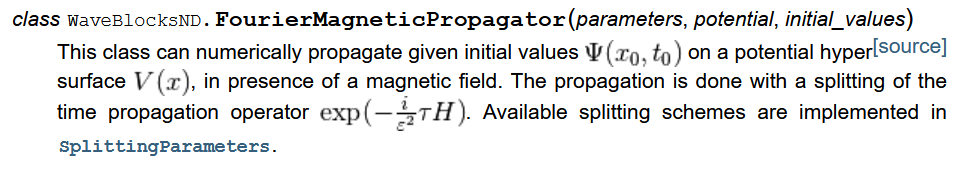
\includegraphics[width = 0.9\textwidth]{graphics/doc_fmp.PNG}
  \caption{Header of the FourierMagneticPropagator Class.}
  \label{fig:doc_fmp}
\end{figure}

In this section, we present the \emph{postpropagate}-function which carries the implementation of \cref{sec:intro} and explain its approach. \newline

The code of the \emph{postpropagate}-function is summarised in Alg. (\ref{alg:postpropagate}). It is based on the algorithm from \defaultcite{GR18}. Its header is visible in \cref{fig:pp}.
\begin{figure}[ht]
  \centering
  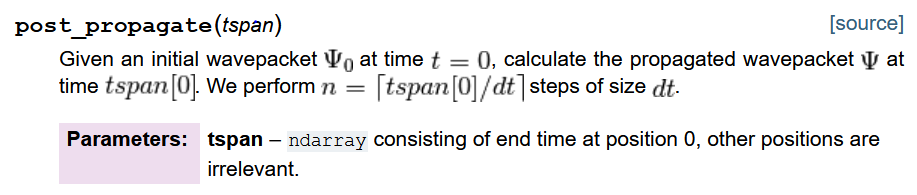
\includegraphics[width = 0.9 \textwidth]{graphics/doc_postpropagate.PNG}
  \caption{Header of the postpropagate-function.}
  \label{fig:pp}
\end{figure}

The flow map $\rho$ from \cref{eq_rho} effectively acts as a rotation. These rotations could not directly be applied onto the potential $V$ or the wavefunction $\Psi$ but had to be realised via a rotation of the underlying grid $X$. More precisely, the operation $(\rho(R)A)(x) = A(R^{-1}x)$ requires us to first rotate the grid $X$ by $R^{-1}$ and then evaluate quantity $A$ on the rotated grid. Because $X$ is a class member in WaveBlocksND, after the evaluation of $A$ on $R^{-1}\cdot X$ the above rotation needs to be reversed to return to the original state. Otherwise subsequent evaluations would be conducted on the wrong grid.\newline
Because of the rotational invariance of the first term in \cref{eq:rotinv}, only the second term $\phi(x,s) + V_{ext}(x,s)$ needs to be subjected to such a rotation. \newline

\begin{algorithm}[H]
  \label{alg:postpropagate}
    \SetAlgoLined
    \caption{PostPropagate Function}
    \BlankLine

    \KwData{\emph{As arguments to the function:} class instance $self$; end time $t$.\newline \emph{As arguments to the class instance:} step width $dt$; meshgrid $X$; initial wave function $\Psi_0$; potential $V$; magnetic field $B$; number of components of the wavefunction $N$; scaled Planck constant $\epsilon$; splitting method with coefficients $(a_i, b_i)_{i = 1}^n$; end time of simulation $T$; dimension $d$; frequency of writing to disk $w_n$.}
    \KwResult{ Computes wavepacket at time $t$ and saves it to class member. Returns End time $t$.}

    define stepwidth: $n_{steps}$ = $\lceil t / dt \rceil $\;
    define time grids: $t_a = t_0$, $t_b = t_0$ \;
    calculate flow map $R = U(t_0 + N\cdot dt, t_0)$ \;
    rotate the grid by $R^T$ \;
    evaluate initial data on rotated grid and save to wavefunction $\Psi$\;
    rotate grid by $R$ \;

    \For{j = 0 to nsteps}{
      \For{i = 0 to dim(a)}{
        potential propagator $\Phi_V = \Phi_{B} \cdot \Phi_{\phi}:$ \\{
          \Indp calculate magnetic field propagator $\Phi_{B} = \exp(-i \langle x, (\int_{t_a}^{t_a + a_i \cdot dt} B^2(s) ds)x \rangle)$ \;
          apply propagator to $\Psi$ \;
          rotate grid by $R^T$ \;
          calculate electric and external potential propagator $\Phi_{\phi} = \exp(-i \int_{t_a}^{t_a + a_i \cdot dt} (\phi(x,s) + V_{ext}) ds)$ \;
          apply propagator to $\Psi$ on rotated grid \;
          rotate grid back \;
        }
        calculate flow map $R = R\cdot U^{-1}(t_b + b_i \cdot dt, t_b)$ \;
        kinetic propagator $\Phi_{-\Delta}$: \\
        {
          \Indp Fast-Fourier-Transform $\Psi$ to Fourier space \;
          calculate the kinetic propagator $\Phi_{-\Delta}$ \;
          apply propagator to $\mathcal{FFT}(\Psi)$ \;
          Inverse-FFT $\Psi$ to real space \;
        }
        update time grids: $t_a = t_a + a_i \cdot dt$, $t_b = t_b + b_i \cdot dt$ \;
      }
    }
    \Return{t}

\end{algorithm}


\section{Results}
In order to investigate the results of the \emph{FourierMagneticPropagator}, we will present two examples and analyse several important metrics, mainly those of energy conservation, norm conservation and convergence. Additionally, the time evolution is shown in appendix \ref{appendix:evolution}.

\subsection{Example: Threefold Morse Potential}
Consider the threefold morse potential for $x \in \mathbb{R}^2$:
\begin{equation*}
  V_{ext}(x) = 8 \left(1 - \exp\left( - \frac{\lVert x \rVert _{\mathbb{R}^2}^2}{32}(1 - \cos(3arctan2(x_2, x_1)))^2\right)\right)^2
\end{equation*}
and the inital data
\begin{equation*}
  \Psi_0^{\epsilon}[q, p, Q, P] = \left( \pi \epsilon^2 Q^2 \right)^{-\frac{1}{4}} \exp \left( \frac{i}{2\epsilon^2} PQ^{-1}(x-q)^2 + \frac{i}{\epsilon^2}p(x-q) \right)
\end{equation*}
 with the parameters from \cref{tab:params}. Note that this corresponds to a wavefunction concentrated in position around $q$ and in momentum around $p$ with uncertainties $\epsilon \lvert Q \rvert / \sqrt{2}$ and $\epsilon \lvert P \rvert / \sqrt{2}$. Additionally consider the step width $dt=0.01$, start time $t_0=0$, end time $T=5$ and the homogeneous, time-independent magnetic field $B = \begin{pmatrix} 0 & -0.5 \\ 0.5 & 0 \end{pmatrix}$. As the splitting method we chose Strang Splitting \defaultcite{G68}.
\begin{table}[h]
  \centering
  \begin{tabular}{c|c}
    q & $\begin{pmatrix}1.0 & 0.0 \end{pmatrix}$ \\ \hline
    p & $\begin{pmatrix}0.0 & 0.0 \end{pmatrix}$ \\ \hline
    Q & $\begin{pmatrix}
      \sqrt{2.0 \cdot 0.56} & 0.0 \\
      0.0 & \sqrt{2.0 \cdot 0.24}
    \end{pmatrix}$ \\ \hline
    P & $\begin{pmatrix}
      i/\sqrt{2.0 \cdot 0.56} & 0.0 \\
      0.0 & i/\sqrt{2.0 \cdot 0.24}
    \end{pmatrix}$ \\
  \end{tabular}
  \caption{Parameters for the initial wavepacket $\Psi_0$.}
  \label{tab:params}

\end{table}
The scaled Planck's constant was set to $\epsilon = 0.25$.
\subsubsection{Energy and Norm conservation}
The evolution of the energies is visible in \cref{fig:threefold_energy}, the evolution of the norms in \cref{fig:threefold_norm}. We found that both energies and norms are approximately constant.
\begin{figure}[h]
  \begin{subfigure}[b]{0.45 \textwidth}
    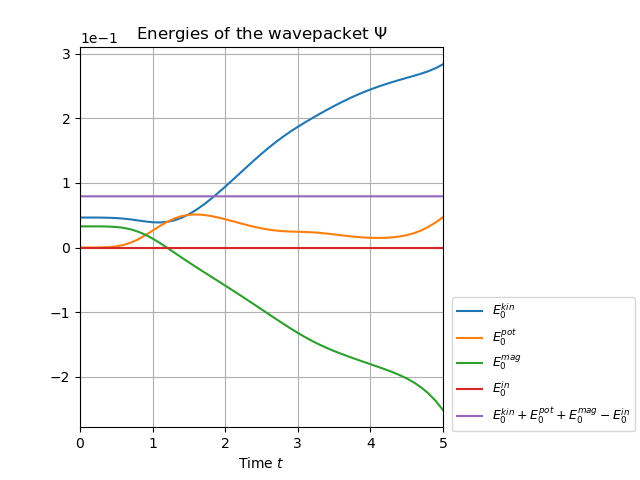
\includegraphics[width = \textwidth]{graphics/threefold_morse/threefold_energies_block0.PNG}
  \end{subfigure}
  \hfill
  \begin{subfigure}[b]{0.45 \textwidth}
    \includegraphics[width = \textwidth]{graphics/threefold_morse/energy_drift_block0_log.PNG}
  \end{subfigure}
  \caption{Energy and energy drift, $\epsilon = 0.25$.}
  \label{fig:threefold_energy}
\end{figure}

\begin{figure}[h]
  \begin{subfigure}[b]{0.45 \textwidth}
    \includegraphics[width = \textwidth]{graphics/threefold_morse/norms_block0.PNG}
  \end{subfigure}
  \hfill
  \begin{subfigure}[b]{0.45 \textwidth}
    \includegraphics[width = \textwidth]{graphics/threefold_morse/norms_drift_block0_log.PNG}
  \end{subfigure}
  \caption{Norm and norm drift, $\epsilon = 0.25$.}
  \label{fig:threefold_norm}
\end{figure}

\begin{figure}[h!]
  \begin{subfigure}[b]{0.45 \textwidth}
    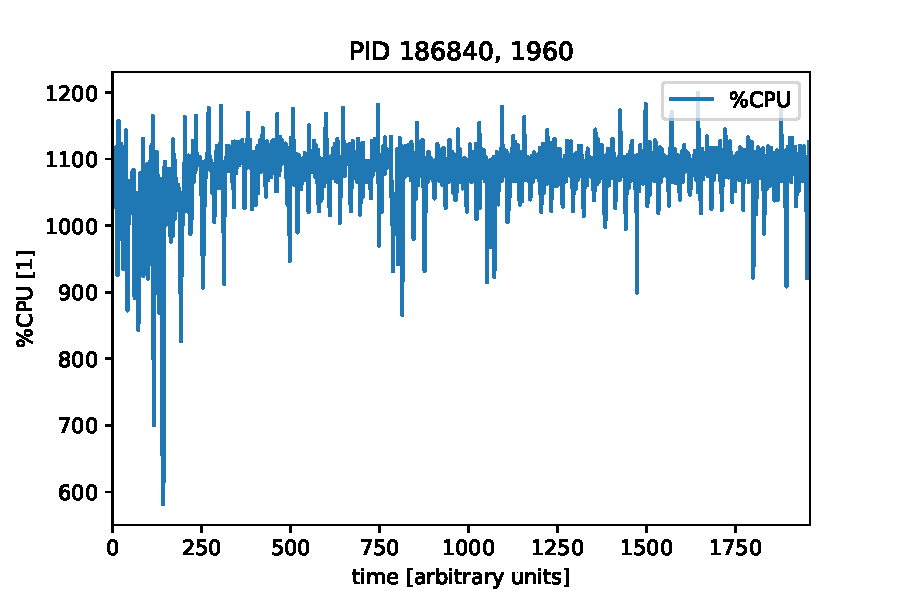
\includegraphics[width = \textwidth]{graphics/threefold_morse/threefold_perCPU.pdf}
    \caption{Percentage of CPU.}
  \end{subfigure}
  ~
  \begin{subfigure}[b]{0.45 \textwidth}
    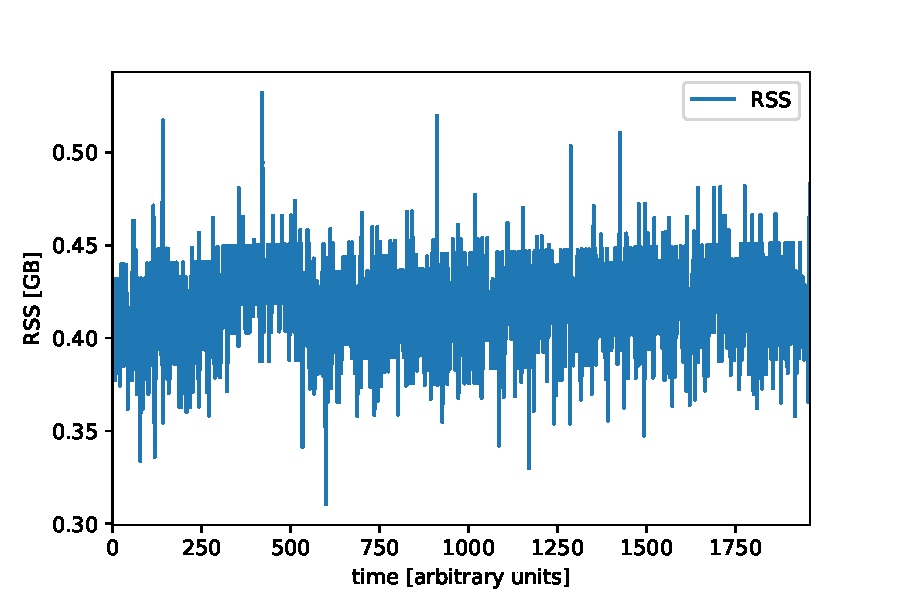
\includegraphics[width = \textwidth]{graphics/threefold_morse/threefold_RSS.pdf}
    \caption{RSS (Resident Set Size).}
  \end{subfigure}
  ~
  \begin{subfigure}[b]{0.45 \textwidth}
    \centering
    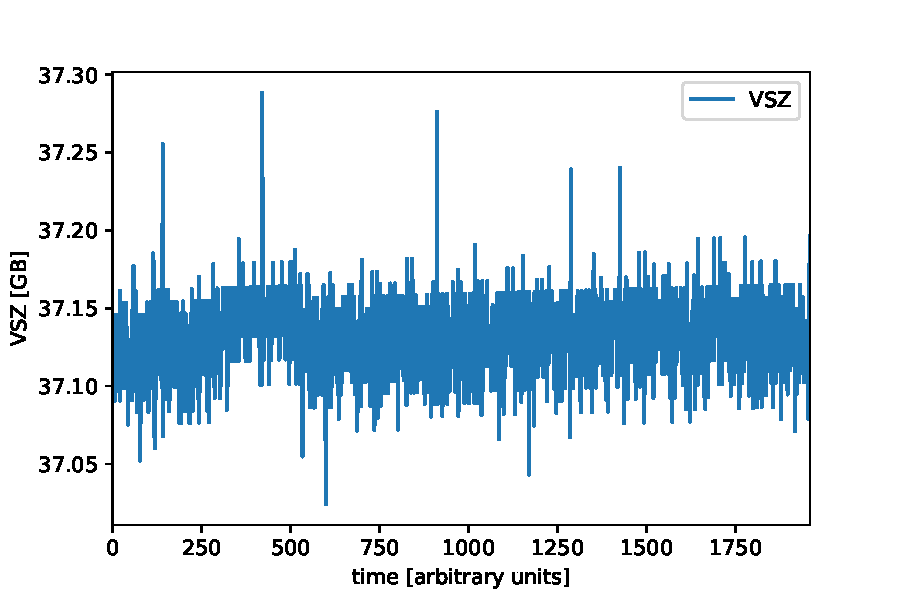
\includegraphics[width = \textwidth]{graphics/threefold_morse/threefold_VSZ.pdf}
    \caption{VSZ (Virtual Memory Size).}
  \end{subfigure}
  \caption{Resource consumption of the simulation with the threefold morse potential.}
  \label{fig:threefold_resource}
\end{figure}

\subsubsection{Resource Consumption}
We ran the simulation on a CPU consisting of 2x AMD Opteron(tm) Processor 6174 with 24 Cores and recorded the resource consumption using Linux' pidstat and time commands. The simulation lasted a total of 5:50:44 (h:min:s) consuming on average $1068 \%$ CPU. The usage of RSS, VSZ and CPU over time is visible in \cref{fig:threefold_resource}.


\subsubsection{Convergence} \label{sec:threefold_conv}
To determine performance for different $\epsilon$, we ran a reference simulation using a splitting of order 6 proposed by Blanes and Moan \defaultcite{BLANES2002313} and a sample simulation using Strang splitting \defaultcite{G68}, which is of order 2. The difference of those simulations for several values of $\epsilon$ is portrayed in \cref{fig:convthreefold}.
\begin{figure}[h]
  \centering
  \includegraphics[width = 110mm]{../../convergence/threefold/coeffdiff.png}
  \caption{Error of the coefficient vectors for different $\epsilon$.}
  \label{fig:convthreefold}
\end{figure}

\subsection{Example: Torsional Potential}
Consider the torsional potential from \defaultcite{FGL09} for $x \in \mathbb{R}^2$:
\begin{equation*}
  V_{ext}(x) = \sum_{i=1}^2 1 - \cos(x_i).
\end{equation*}
Consider $\Psi_0$ to be as in the example above with the parameters from \cref{tab:params}, $\epsilon = 0.25$ and the splitting to be Strang Splitting \defaultcite{G68}.

\subsubsection{Energy and Norm conservation}
The energy and norm evolution over time is depicted in \cref{fig:cos_energy} and \cref{fig:cos_norm} respectively.

\begin{figure}[h]
  \begin{subfigure}[b]{0.45 \textwidth}
    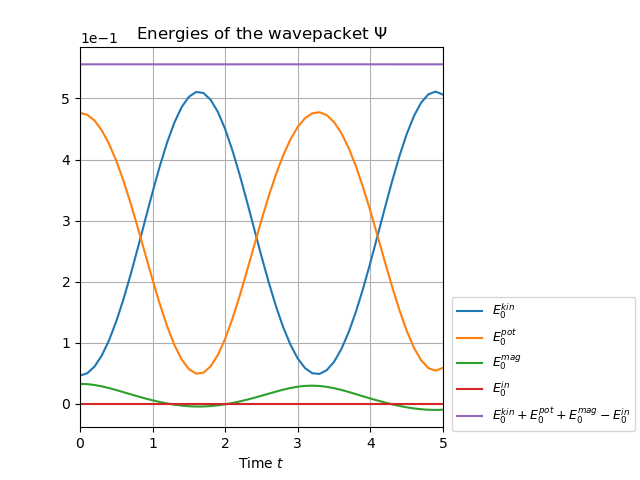
\includegraphics[width = \textwidth]{graphics/torsional/energies_block0.PNG}
  \end{subfigure}
  \hfill
  \begin{subfigure}[b]{0.45 \textwidth}
    \includegraphics[width = \textwidth]{graphics/torsional/energy_drift_block0_log.PNG}
  \end{subfigure}
  \caption{Energy and energy drift, $\epsilon = 0.25$.}
  \label{fig:cos_energy}
\end{figure}

\begin{figure}[h]
  \begin{subfigure}[b]{0.45 \textwidth}
    \includegraphics[width = \textwidth]{graphics/torsional/norms_block0.PNG}
  \end{subfigure}
  \hfill
  \begin{subfigure}[b]{0.45 \textwidth}
    \includegraphics[width = \textwidth]{graphics/torsional/norms_drift_block0_log.PNG}
  \end{subfigure}
  \caption{Norm and norm drift, $\epsilon = 0.25$.}
  \label{fig:cos_norm}
\end{figure}


\subsubsection{Resource Consumption}
We ran the simulation on a setup identical to the one mentioned above and again recorded the resource consumpion using Linux' time and pidstat commands. The simulation lasted for a total of 7:45:18 (h:min:s) and consumed $247 \%$ CPU. The usage of RSS, VSZ and CPU over time is visible in \cref{fig:cos_resource}.
\begin{figure}[h]
  \begin{subfigure}[b]{0.45 \textwidth}
    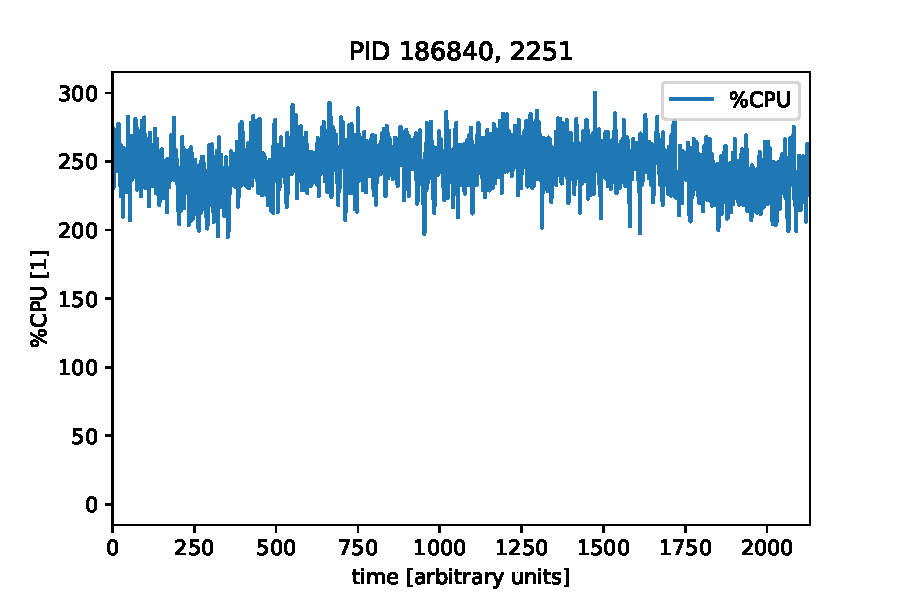
\includegraphics[width = \textwidth]{../parser/cospot_perCPU.pdf}
    \caption{Percentage of CPU.}
  \end{subfigure}
  ~
  \begin{subfigure}[b]{0.45 \textwidth}
    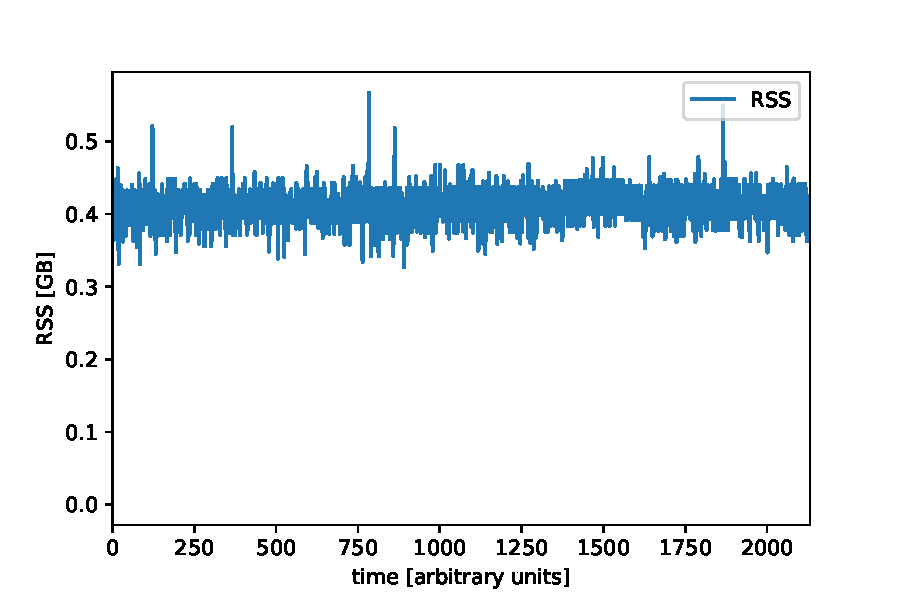
\includegraphics[width = \textwidth]{../parser/cospot_RSS.pdf}
    \caption{RSS (Resident Set Size).}
  \end{subfigure}
  ~
  \begin{subfigure}[b]{0.45 \textwidth}
    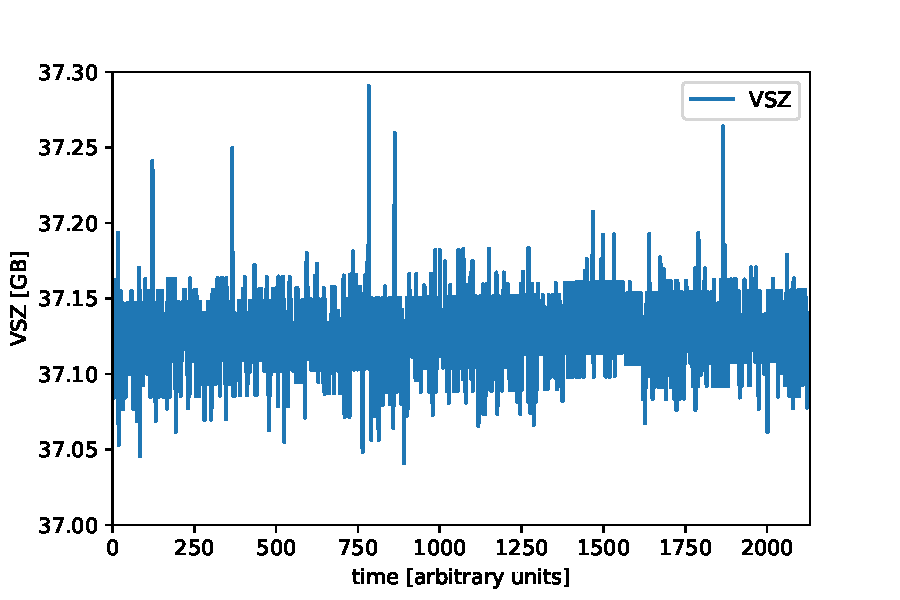
\includegraphics[width = \textwidth]{../parser/cospot_VSZ.pdf}
    \caption{VSZ (Virtual Memory Size).}
  \end{subfigure}
  \caption{Resource consumption of the simulation with the torsional potential. The difference in CPU percentage between the torsional potential and the morse potential is mostly due to different loads on the machines at the time of simulation.}
  \label{fig:cos_resource}
\end{figure}


\subsubsection{Convergence}
The same considerations as in \cref{sec:threefold_conv} were made for the torsional potential. The difference of those simulations for various values of $\epsilon$ is portrayed in \cref{fig:convtorsional}.
\begin{figure}[H]
  \centering
  \includegraphics[width = 110mm]{../../convergence/torsional/coeffdiff.png}
  \caption{Error of the coefficient vectors for different $\epsilon$.}
  \label{fig:convtorsional}
\end{figure}

\section{Discussion and Conclusion}
In the course of this semester thesis, we implemented the method developed by Rietmann and Gradinaru in \defaultcite{GR18} into the WaveblocksND framework. We found that energies and norms are conserved well in both of the cases we explored.
From \cref{fig:convthreefold} and \cref{fig:convtorsional} we can conclude that the method is well suited for values of $\epsilon > 0.125$, but is prone to much larger errors for values of $\epsilon$ smaller than that.\newline
One major disadvantage of this method is its speed. Simulations are time- and resource intensive. Additionally the structure of the method results in the fact that time-steps are not consecutive but have to be calculated individually. I.e. to write data to the disk after the 10th and 20th time step (for example to calculate the energy at those times) the simulation needs to run the first 10 time-steps, write to disk, restart at $t_0$ and run the first 20 time-steps. This doesn't present itself as a problem when only the state at a certain end-time $T$ is needed but quickly becomes costly if a high resolution in the time-steps is required.

For further research, one could investigate the performance of this method for a particle in a time-dependent magnetic field as well as in dimensions $d > 2$. Additionally performance could be compared to the semi-classical wavepacket approach from \defaultcite{FGL09} also implemented in WaveBlocksND.


\begin{appendices}


\section{Code} \label{appendix:code}

%%\inputminted{python}{../FourierMagneticPropagator.py}

%% make sure to refresh this at the end

\lstinputlisting[language=Python]{../FourierMagneticPropagator.py}

%%\begin{Verbatim}[commandchars=\\\{\}]
\PY{l+s+sa}{r}\PY{l+s+sd}{\PYZdq{}\PYZdq{}\PYZdq{}The WaveBlocks Project}

\PY{l+s+sd}{This file contains the Fourier Magnetic Propagator class. The wavefunction}
\PY{l+s+sd}{:math:`\PYZbs{}Psi` is propagated in time with a splitting of the}
\PY{l+s+sd}{exponential :math:`\PYZbs{}exp(\PYZhy{}\PYZbs{}frac\PYZob{}i\PYZcb{}\PYZob{}\PYZbs{}varepsilon\PYZca{}2\PYZcb{} \PYZbs{}tau H)`.}

\PY{l+s+sd}{@author: R. Bourquin}
\PY{l+s+sd}{@copyright: Copyright (C) 2012, 2016 R. Bourquin}
\PY{l+s+sd}{@license: Modified BSD License}
\PY{l+s+sd}{\PYZdq{}\PYZdq{}\PYZdq{}}

\PY{k+kn}{from} \PY{n+nn}{numpy} \PY{k+kn}{import} \PY{n}{array}\PY{p}{,} \PY{n}{complexfloating}\PY{p}{,} \PY{n}{dot}\PY{p}{,} \PY{n}{exp}\PY{p}{,} \PY{n}{eye}\PY{p}{,} \PY{n}{zeros}\PY{p}{,} \PY{n}{shape}
\PY{k+kn}{from} \PY{n+nn}{numpy.fft} \PY{k+kn}{import} \PY{n}{fftn}\PY{p}{,} \PY{n}{ifftn}
\PY{k+kn}{from} \PY{n+nn}{scipy.linalg} \PY{k+kn}{import} \PY{n}{expm}

\PY{k+kn}{from} \PY{n+nn}{WaveBlocksND.BlockFactory} \PY{k+kn}{import} \PY{n}{BlockFactory}
\PY{k+kn}{from} \PY{n+nn}{WaveBlocksND.Propagator} \PY{k+kn}{import} \PY{n}{Propagator}
\PY{k+kn}{from} \PY{n+nn}{WaveBlocksND.KineticOperator} \PY{k+kn}{import} \PY{n}{KineticOperator}
\PY{k+kn}{from} \PY{n+nn}{WaveBlocksND.MagneticField} \PY{k+kn}{import} \PY{n}{MagneticField}
\PY{k+kn}{from} \PY{n+nn}{WaveBlocksND.SplittingParameters} \PY{k+kn}{import} \PY{n}{SplittingParameters}

\PY{n}{\PYZus{}\PYZus{}all\PYZus{}\PYZus{}} \PY{o}{=} \PY{p}{[}\PY{l+s+s2}{\PYZdq{}}\PY{l+s+s2}{FourierMagneticPropagator}\PY{l+s+s2}{\PYZdq{}}\PY{p}{]}


\PY{k}{class} \PY{n+nc}{FourierMagneticPropagator}\PY{p}{(}\PY{n}{Propagator}\PY{p}{,} \PY{n}{SplittingParameters}\PY{p}{)}\PY{p}{:}
    \PY{l+s+sa}{r}\PY{l+s+sd}{\PYZdq{}\PYZdq{}\PYZdq{}This class can numerically propagate given initial values :math:`\PYZbs{}Psi(x\PYZus{}0, t\PYZus{}0)` on}
\PY{l+s+sd}{    a potential hyper surface :math:`V(x)`, in presence of a magnetic field. The propagation is done with a splitting}
\PY{l+s+sd}{    of the time propagation operator :math:`\PYZbs{}exp(\PYZhy{}\PYZbs{}frac\PYZob{}i\PYZcb{}\PYZob{}\PYZbs{}varepsilon\PYZca{}2\PYZcb{} \PYZbs{}tau H)`.}
\PY{l+s+sd}{    Available splitting schemes are implemented in :py:class:`SplittingParameters`.}
\PY{l+s+sd}{    \PYZdq{}\PYZdq{}\PYZdq{}}

    \PY{k}{def} \PY{n+nf+fm}{\PYZus{}\PYZus{}init\PYZus{}\PYZus{}}\PY{p}{(}\PY{n+nb+bp}{self}\PY{p}{,} \PY{n}{parameters}\PY{p}{,} \PY{n}{potential}\PY{p}{,} \PY{n}{initial\PYZus{}values}\PY{p}{)}\PY{p}{:}
        \PY{l+s+sa}{r}\PY{l+s+sd}{\PYZdq{}\PYZdq{}\PYZdq{}Initialize a new :py:class:`FourierMagneticPropagator` instance. Precalculate the}
\PY{l+s+sd}{        the kinetic operator :math:`T\PYZus{}e` and the potential operator :math:`V\PYZus{}e`}
\PY{l+s+sd}{        used for time propagation.}

\PY{l+s+sd}{        :param parameters: The set of simulation parameters. It must contain at least}
\PY{l+s+sd}{                           the semi\PYZhy{}classical parameter :math:`\PYZbs{}varepsilon` and the}
\PY{l+s+sd}{                           time step size :math:`\PYZbs{}tau`.}
\PY{l+s+sd}{        :param potential: The potential :math:`V(x)` governing the time evolution.}
\PY{l+s+sd}{        :type potential: A :py:class:`MatrixPotential` instance.}
\PY{l+s+sd}{        :param initial\PYZus{}values: The initial values :math:`\PYZbs{}Psi(\PYZbs{}Gamma, t\PYZus{}0)` given}
\PY{l+s+sd}{                               in the canonical basis.}
\PY{l+s+sd}{        :type initial\PYZus{}values: A :py:class:`WaveFunction` instance.}

\PY{l+s+sd}{        :raise: :py:class:`ValueError` If the number of components of :math:`\PYZbs{}Psi` does not match the}
\PY{l+s+sd}{                           number of energy surfaces :math:`\PYZbs{}lambda\PYZus{}i(x)` of the potential.}

\PY{l+s+sd}{        :raise: :py:class:`ValueError` If the number of components of :math:`\PYZbs{}Psi` does not match the dimension of the magnetic field :math:`\PYZbs{}vec\PYZob{}B\PYZcb{}(x)`.}

\PY{l+s+sd}{        :raise: :py:class:`ValueError` If the dimensions of the splitting scheme parameters :math:`a` and :math:`b` are not equal.}
\PY{l+s+sd}{        \PYZdq{}\PYZdq{}\PYZdq{}}
        \PY{c+c1}{\PYZsh{} The embedded \PYZsq{}MatrixPotential\PYZsq{} instance representing the potential \PYZsq{}V\PYZsq{}.}
        \PY{n+nb+bp}{self}\PY{o}{.}\PY{n}{\PYZus{}potential} \PY{o}{=} \PY{n}{potential}

        \PY{c+c1}{\PYZsh{} The initial values of the components \PYZsq{}\PYZbs{}psi\PYZus{}i\PYZsq{} sampled at the given grid.}
        \PY{n+nb+bp}{self}\PY{o}{.}\PY{n}{\PYZus{}psi} \PY{o}{=} \PY{n}{initial\PYZus{}values}

        \PY{k}{if} \PY{n+nb+bp}{self}\PY{o}{.}\PY{n}{\PYZus{}potential}\PY{o}{.}\PY{n}{get\PYZus{}number\PYZus{}components}\PY{p}{(}\PY{p}{)} \PY{o}{!=} \PY{n+nb+bp}{self}\PY{o}{.}\PY{n}{\PYZus{}psi}\PY{o}{.}\PY{n}{get\PYZus{}number\PYZus{}components}\PY{p}{(}\PY{p}{)}\PY{p}{:}
            \PY{k}{raise} \PY{n+ne}{ValueError}\PY{p}{(}\PY{l+s+s2}{\PYZdq{}}\PY{l+s+s2}{Potential dimension and number of components do not match.}\PY{l+s+s2}{\PYZdq{}}\PY{p}{)}

        \PY{c+c1}{\PYZsh{} The time step size.}
        \PY{n+nb+bp}{self}\PY{o}{.}\PY{n}{\PYZus{}dt} \PY{o}{=} \PY{n}{parameters}\PY{p}{[}\PY{l+s+s2}{\PYZdq{}}\PY{l+s+s2}{dt}\PY{l+s+s2}{\PYZdq{}}\PY{p}{]}

        \PY{c+c1}{\PYZsh{} Final time.}
        \PY{n+nb+bp}{self}\PY{o}{.}\PY{n}{\PYZus{}T} \PY{o}{=} \PY{n}{parameters}\PY{p}{[}\PY{l+s+s2}{\PYZdq{}}\PY{l+s+s2}{T}\PY{l+s+s2}{\PYZdq{}}\PY{p}{]}

        \PY{c+c1}{\PYZsh{} The model parameter \PYZsq{}\PYZbs{}varepsilon\PYZsq{}.}
        \PY{n+nb+bp}{self}\PY{o}{.}\PY{n}{\PYZus{}eps} \PY{o}{=} \PY{n}{parameters}\PY{p}{[}\PY{l+s+s2}{\PYZdq{}}\PY{l+s+s2}{eps}\PY{l+s+s2}{\PYZdq{}}\PY{p}{]}

        \PY{c+c1}{\PYZsh{} Spacial dimension d}
        \PY{n+nb+bp}{self}\PY{o}{.}\PY{n}{\PYZus{}dimension} \PY{o}{=} \PY{n}{parameters}\PY{p}{[}\PY{l+s+s2}{\PYZdq{}}\PY{l+s+s2}{dimension}\PY{l+s+s2}{\PYZdq{}}\PY{p}{]}

        \PY{c+c1}{\PYZsh{} The position space grid nodes \PYZsq{}\PYZbs{}Gamma\PYZsq{}.}
        \PY{n+nb+bp}{self}\PY{o}{.}\PY{n}{\PYZus{}grid} \PY{o}{=} \PY{n}{initial\PYZus{}values}\PY{o}{.}\PY{n}{get\PYZus{}grid}\PY{p}{(}\PY{p}{)}

        \PY{c+c1}{\PYZsh{} The kinetic operator \PYZsq{}T\PYZsq{} defined in momentum space.}
        \PY{n+nb+bp}{self}\PY{o}{.}\PY{n}{\PYZus{}KO} \PY{o}{=} \PY{n}{KineticOperator}\PY{p}{(}\PY{n+nb+bp}{self}\PY{o}{.}\PY{n}{\PYZus{}grid}\PY{p}{,} \PY{n+nb+bp}{self}\PY{o}{.}\PY{n}{\PYZus{}eps}\PY{p}{)}

        \PY{c+c1}{\PYZsh{} Exponential \PYZsq{}\PYZbs{}exp(\PYZhy{}i/2*eps\PYZca{}2*dt*T)\PYZsq{} used in the Strang splitting.}
        \PY{c+c1}{\PYZsh{} not used}
        \PY{n+nb+bp}{self}\PY{o}{.}\PY{n}{\PYZus{}KO}\PY{o}{.}\PY{n}{calculate\PYZus{}exponential}\PY{p}{(}\PY{o}{\PYZhy{}}\PY{l+m+mf}{0.5j} \PY{o}{*} \PY{n+nb+bp}{self}\PY{o}{.}\PY{n}{\PYZus{}dt} \PY{o}{*} \PY{n+nb+bp}{self}\PY{o}{.}\PY{n}{\PYZus{}eps}\PY{o}{*}\PY{o}{*}\PY{l+m+mi}{2}\PY{p}{)}
        \PY{n+nb+bp}{self}\PY{o}{.}\PY{n}{\PYZus{}TE} \PY{o}{=} \PY{n+nb+bp}{self}\PY{o}{.}\PY{n}{\PYZus{}KO}\PY{o}{.}\PY{n}{evaluate\PYZus{}exponential\PYZus{}at}\PY{p}{(}\PY{p}{)}

        \PY{c+c1}{\PYZsh{} Exponential \PYZsq{}\PYZbs{}exp(\PYZhy{}i/eps\PYZca{}2*dt*V)\PYZsq{} used in the Strang splitting.}
        \PY{c+c1}{\PYZsh{} not used}
        \PY{n+nb+bp}{self}\PY{o}{.}\PY{n}{\PYZus{}potential}\PY{o}{.}\PY{n}{calculate\PYZus{}exponential}\PY{p}{(}\PY{o}{\PYZhy{}}\PY{l+m+mf}{0.5j} \PY{o}{*} \PY{n+nb+bp}{self}\PY{o}{.}\PY{n}{\PYZus{}dt} \PY{o}{/} \PY{n+nb+bp}{self}\PY{o}{.}\PY{n}{\PYZus{}eps}\PY{o}{*}\PY{o}{*}\PY{l+m+mi}{2}\PY{p}{)}
        \PY{n}{VE} \PY{o}{=} \PY{n+nb+bp}{self}\PY{o}{.}\PY{n}{\PYZus{}potential}\PY{o}{.}\PY{n}{evaluate\PYZus{}exponential\PYZus{}at}\PY{p}{(}\PY{n+nb+bp}{self}\PY{o}{.}\PY{n}{\PYZus{}grid}\PY{p}{)}
        \PY{n+nb+bp}{self}\PY{o}{.}\PY{n}{\PYZus{}VE} \PY{o}{=} \PY{n+nb}{tuple}\PY{p}{(}\PY{p}{[}\PY{n}{ve}\PY{o}{.}\PY{n}{reshape}\PY{p}{(}\PY{n+nb+bp}{self}\PY{o}{.}\PY{n}{\PYZus{}grid}\PY{o}{.}\PY{n}{get\PYZus{}number\PYZus{}nodes}\PY{p}{(}\PY{p}{)}\PY{p}{)} \PY{k}{for} \PY{n}{ve} \PY{o+ow}{in} \PY{n}{VE}\PY{p}{]}\PY{p}{)}

        \PY{c+c1}{\PYZsh{} The magnetic field}
        \PY{n+nb+bp}{self}\PY{o}{.}\PY{n}{\PYZus{}B} \PY{o}{=} \PY{n}{MagneticField}\PY{p}{(}\PY{n}{parameters}\PY{p}{[}\PY{l+s+s2}{\PYZdq{}}\PY{l+s+s2}{B}\PY{l+s+s2}{\PYZdq{}}\PY{p}{]}\PY{p}{)}
        \PY{c+c1}{\PYZsh{} check if magnetic field and potential are of same dimension}
        \PY{k}{if} \PY{n+nb+bp}{self}\PY{o}{.}\PY{n}{\PYZus{}B}\PY{o}{.}\PY{n}{get\PYZus{}dimension}\PY{p}{(}\PY{p}{)} \PY{o}{!=} \PY{n+nb+bp}{self}\PY{o}{.}\PY{n}{\PYZus{}dimension}\PY{p}{:}
            \PY{k}{raise} \PY{n+ne}{ValueError}\PY{p}{(}\PY{l+s+s2}{\PYZdq{}}\PY{l+s+s2}{Spacial dimension of potential and magnetic field must be the same}\PY{l+s+s2}{\PYZdq{}}\PY{p}{)}

        \PY{c+c1}{\PYZsh{}precalculate the splitting needed}
        \PY{n+nb+bp}{self}\PY{o}{.}\PY{n}{\PYZus{}a}\PY{p}{,} \PY{n+nb+bp}{self}\PY{o}{.}\PY{n}{\PYZus{}b} \PY{o}{=} \PY{n+nb+bp}{self}\PY{o}{.}\PY{n}{build}\PY{p}{(}\PY{n}{parameters}\PY{p}{[}\PY{l+s+s2}{\PYZdq{}}\PY{l+s+s2}{splitting\PYZus{}method}\PY{l+s+s2}{\PYZdq{}}\PY{p}{]}\PY{p}{)}
        \PY{k}{if} \PY{n}{shape}\PY{p}{(}\PY{n+nb+bp}{self}\PY{o}{.}\PY{n}{\PYZus{}a}\PY{p}{)} \PY{o}{!=} \PY{n}{shape}\PY{p}{(}\PY{n+nb+bp}{self}\PY{o}{.}\PY{n}{\PYZus{}b}\PY{p}{)}\PY{p}{:}
            \PY{k}{raise} \PY{n+ne}{ValueError}\PY{p}{(}\PY{l+s+s2}{\PYZdq{}}\PY{l+s+s2}{Splitting scheme shapes must be the same}\PY{l+s+s2}{\PYZdq{}}\PY{p}{)}

        \PY{c+c1}{\PYZsh{} Get inital data as function}
        \PY{n}{packet\PYZus{}descr} \PY{o}{=} \PY{n}{parameters}\PY{p}{[}\PY{l+s+s2}{\PYZdq{}}\PY{l+s+s2}{initvals}\PY{l+s+s2}{\PYZdq{}}\PY{p}{]}\PY{p}{[}\PY{l+m+mi}{0}\PY{p}{]}
        \PY{n+nb+bp}{self}\PY{o}{.}\PY{n}{\PYZus{}initalpacket} \PY{o}{=} \PY{n}{BlockFactory}\PY{p}{(}\PY{p}{)}\PY{o}{.}\PY{n}{create\PYZus{}wavepacket}\PY{p}{(}\PY{n}{packet\PYZus{}descr}\PY{p}{)}


    \PY{c+c1}{\PYZsh{} TODO: Consider removing this, duplicate}
    \PY{k}{def} \PY{n+nf}{get\PYZus{}number\PYZus{}components}\PY{p}{(}\PY{n+nb+bp}{self}\PY{p}{)}\PY{p}{:}
        \PY{l+s+sa}{r}\PY{l+s+sd}{\PYZdq{}\PYZdq{}\PYZdq{}Get the number :math:`N` of components of :math:`\PYZbs{}Psi`.}

\PY{l+s+sd}{        :return: The number :math:`N`.}
\PY{l+s+sd}{        \PYZdq{}\PYZdq{}\PYZdq{}}
        \PY{k}{return} \PY{n+nb+bp}{self}\PY{o}{.}\PY{n}{\PYZus{}potential}\PY{o}{.}\PY{n}{get\PYZus{}number\PYZus{}components}\PY{p}{(}\PY{p}{)}


    \PY{k}{def} \PY{n+nf}{get\PYZus{}wavefunction}\PY{p}{(}\PY{n+nb+bp}{self}\PY{p}{)}\PY{p}{:}
        \PY{l+s+sa}{r}\PY{l+s+sd}{\PYZdq{}\PYZdq{}\PYZdq{}Get the wavefunction that stores the current data :math:`\PYZbs{}Psi(\PYZbs{}Gamma)`.}

\PY{l+s+sd}{        :return: The :py:class:`WaveFunction` instance.}
\PY{l+s+sd}{        \PYZdq{}\PYZdq{}\PYZdq{}}
        \PY{k}{return} \PY{n+nb+bp}{self}\PY{o}{.}\PY{n}{\PYZus{}psi}


    \PY{k}{def} \PY{n+nf}{get\PYZus{}operators}\PY{p}{(}\PY{n+nb+bp}{self}\PY{p}{)}\PY{p}{:}
        \PY{l+s+sa}{r}\PY{l+s+sd}{\PYZdq{}\PYZdq{}\PYZdq{}Get the kinetic and potential operators :math:`T(\PYZbs{}Omega)` and :math:`V(\PYZbs{}Gamma)`.}

\PY{l+s+sd}{        :return: A tuple :math:`(T, V)` containing two ``ndarrays``.}
\PY{l+s+sd}{        \PYZdq{}\PYZdq{}\PYZdq{}}
        \PY{c+c1}{\PYZsh{} TODO: What kind of object exactly do we want to return?}
        \PY{n+nb+bp}{self}\PY{o}{.}\PY{n}{\PYZus{}KO}\PY{o}{.}\PY{n}{calculate\PYZus{}operator}\PY{p}{(}\PY{p}{)}
        \PY{n}{T} \PY{o}{=} \PY{n+nb+bp}{self}\PY{o}{.}\PY{n}{\PYZus{}KO}\PY{o}{.}\PY{n}{evaluate\PYZus{}at}\PY{p}{(}\PY{p}{)}
        \PY{n}{V} \PY{o}{=} \PY{n+nb+bp}{self}\PY{o}{.}\PY{n}{\PYZus{}potential}\PY{o}{.}\PY{n}{evaluate\PYZus{}at}\PY{p}{(}\PY{n+nb+bp}{self}\PY{o}{.}\PY{n}{\PYZus{}grid}\PY{p}{)}
        \PY{n}{V} \PY{o}{=} \PY{n+nb}{tuple}\PY{p}{(}\PY{p}{[}\PY{n}{v}\PY{o}{.}\PY{n}{reshape}\PY{p}{(}\PY{n+nb+bp}{self}\PY{o}{.}\PY{n}{\PYZus{}grid}\PY{o}{.}\PY{n}{get\PYZus{}number\PYZus{}nodes}\PY{p}{(}\PY{p}{)}\PY{p}{)} \PY{k}{for} \PY{n}{v} \PY{o+ow}{in} \PY{n}{V}\PY{p}{]}\PY{p}{)}
        \PY{k}{return} \PY{p}{(}\PY{n}{T}\PY{p}{,} \PY{n}{V}\PY{p}{)}


    \PY{n+nd}{@staticmethod}
    \PY{k}{def} \PY{n+nf}{\PYZus{}Magnus\PYZus{}CF4}\PY{p}{(}\PY{n}{tspan}\PY{p}{,} \PY{n}{B}\PY{p}{,} \PY{n}{N}\PY{p}{,} \PY{o}{*}\PY{n}{args}\PY{p}{)}\PY{p}{:}
        \PY{l+s+sa}{r}\PY{l+s+sd}{\PYZdq{}\PYZdq{}\PYZdq{}Returns the  Fourth Order Magnus integrator :math:`\PYZbs{}Omega(A)` according to [\PYZsh{}]\PYZus{}.}

\PY{l+s+sd}{        :param tspan: Full timespan of expansion.}

\PY{l+s+sd}{        :param B: Magnetic field matrix :math:`B(t) = (B\PYZus{}\PYZob{}j,k\PYZcb{}(t))\PYZus{}\PYZob{}1 \PYZbs{}leq j, k \PYZbs{}leq d\PYZcb{}`.}

\PY{l+s+sd}{        :param N: Number of timesteps for the expansion.}

\PY{l+s+sd}{        :param *args: Additional arguments for the magnetic field :math:`B(t, *args)`}

\PY{l+s+sd}{        .. [\PYZsh{}] S. Blanes and P.C. Moan. \PYZdq{}Fourth\PYZhy{} and sixth\PYZhy{}order commutator\PYZhy{}free Magnus integrators for linear and non\PYZhy{}linear dynamical systems\PYZdq{}. Applied Numerical Mathematics, 56(12):1519 \PYZhy{} 1537, 2006.}
\PY{l+s+sd}{        \PYZdq{}\PYZdq{}\PYZdq{}}
        \PY{c+c1}{\PYZsh{} Magnus constants}
        \PY{n}{c1} \PY{o}{=} \PY{l+m+mf}{0.5}\PY{o}{*}\PY{p}{(}\PY{l+m+mf}{1.0} \PY{o}{\PYZhy{}} \PY{l+m+mf}{0.5773502691896258}\PY{p}{)}
        \PY{n}{c2} \PY{o}{=} \PY{l+m+mf}{0.5}\PY{o}{*}\PY{p}{(}\PY{l+m+mf}{1.0} \PY{o}{+} \PY{l+m+mf}{0.5773502691896258}\PY{p}{)}
        \PY{n}{a1} \PY{o}{=} \PY{l+m+mf}{0.5}\PY{o}{*}\PY{p}{(}\PY{l+m+mf}{0.5} \PY{o}{\PYZhy{}} \PY{l+m+mf}{0.5773502691896258}\PY{p}{)}
        \PY{n}{a2} \PY{o}{=} \PY{l+m+mf}{0.5}\PY{o}{*}\PY{p}{(}\PY{l+m+mf}{0.5} \PY{o}{+} \PY{l+m+mf}{0.5773502691896258}\PY{p}{)}

        \PY{n}{R} \PY{o}{=} \PY{l+m+mf}{1.}\PY{o}{*}\PY{n}{eye}\PY{p}{(} \PY{n+nb}{len}\PY{p}{(} \PY{n}{B}\PY{p}{(}\PY{l+m+mf}{1.}\PY{o}{*}\PY{n}{tspan}\PY{p}{[}\PY{l+m+mi}{0}\PY{p}{]}\PY{p}{,} \PY{o}{*}\PY{n}{args}\PY{p}{)} \PY{p}{)} \PY{p}{)}
        \PY{n}{h} \PY{o}{=} \PY{p}{(}\PY{n}{tspan}\PY{p}{[}\PY{l+m+mi}{1}\PY{p}{]}\PY{o}{\PYZhy{}}\PY{n}{tspan}\PY{p}{[}\PY{l+m+mi}{0}\PY{p}{]}\PY{p}{)} \PY{o}{/} \PY{p}{(}\PY{l+m+mf}{1.}\PY{o}{*}\PY{n}{N}\PY{p}{)}
        \PY{k}{for} \PY{n}{k} \PY{o+ow}{in} \PY{n+nb}{range}\PY{p}{(}\PY{n}{N}\PY{p}{)}\PY{p}{:}
            \PY{n}{t0} \PY{o}{=} \PY{n}{k}\PY{o}{*}\PY{n}{h} \PY{o}{+} \PY{n}{tspan}\PY{p}{[}\PY{l+m+mi}{0}\PY{p}{]}
            \PY{n}{t1} \PY{o}{=} \PY{n}{t0} \PY{o}{+} \PY{n}{c1}\PY{o}{*}\PY{n}{h}
            \PY{n}{t2} \PY{o}{=} \PY{n}{t0} \PY{o}{+} \PY{n}{c2}\PY{o}{*}\PY{n}{h}
            \PY{n}{B1} \PY{o}{=} \PY{n}{B}\PY{p}{(}\PY{n}{t1}\PY{p}{,} \PY{o}{*}\PY{n}{args}\PY{p}{)}
            \PY{n}{B2} \PY{o}{=} \PY{n}{B}\PY{p}{(}\PY{n}{t2}\PY{p}{,} \PY{o}{*}\PY{n}{args}\PY{p}{)}
            \PY{n}{R} \PY{o}{=} \PY{n}{dot}\PY{p}{(}\PY{n}{expm}\PY{p}{(}\PY{n}{a1}\PY{o}{*}\PY{n}{h}\PY{o}{*}\PY{n}{B1}\PY{o}{+}\PY{n}{a2}\PY{o}{*}\PY{n}{h}\PY{o}{*}\PY{n}{B2}\PY{p}{)}\PY{p}{,} \PY{n}{dot}\PY{p}{(}\PY{n}{expm}\PY{p}{(}\PY{n}{a2}\PY{o}{*}\PY{n}{h}\PY{o}{*}\PY{n}{B1}\PY{o}{+}\PY{n}{a1}\PY{o}{*}\PY{n}{h}\PY{o}{*}\PY{n}{B2}\PY{p}{)}\PY{p}{,} \PY{n}{R}\PY{p}{)}\PY{p}{)}

        \PY{k}{return} \PY{n}{R}


    \PY{k}{def} \PY{n+nf}{post\PYZus{}propagate}\PY{p}{(}\PY{n+nb+bp}{self}\PY{p}{,} \PY{n}{tspan}\PY{p}{)}\PY{p}{:}
        \PY{l+s+sa}{r}\PY{l+s+sd}{\PYZdq{}\PYZdq{}\PYZdq{}Given an initial wavepacket :math:`\PYZbs{}Psi\PYZus{}0` at time :math:`t=0`, calculate the propagated wavepacket :math:`\PYZbs{}Psi` at time :math:`tspan \PYZbs{}[ 0 \PYZbs{}]`. We perform :math:`n = \PYZbs{}lceil tspan\PYZbs{}[ 0 \PYZbs{}] /dt \PYZbs{}rceil` steps of size :math:`dt`.}

\PY{l+s+sd}{        :param tspan: :py class:`ndarray` consisting of end time at position 0, other positions are irrelevant.}
\PY{l+s+sd}{        \PYZdq{}\PYZdq{}\PYZdq{}}

        \PY{c+c1}{\PYZsh{} (ignoriere tspan[0])}
        \PY{n}{nsteps} \PY{o}{=} \PY{n+nb}{int}\PY{p}{(}\PY{n}{tspan}\PY{p}{[}\PY{l+m+mi}{0}\PY{p}{]} \PY{o}{/} \PY{n+nb+bp}{self}\PY{o}{.}\PY{n}{\PYZus{}dt} \PY{o}{+} \PY{l+m+mf}{0.5}\PY{p}{)}
        \PY{k}{print}\PY{p}{(}\PY{l+s+s2}{\PYZdq{}}\PY{l+s+s2}{Perform }\PY{l+s+s2}{\PYZdq{}} \PY{o}{+} \PY{n+nb}{str}\PY{p}{(}\PY{n}{nsteps}\PY{p}{)} \PY{o}{+} \PY{l+s+s2}{\PYZdq{}}\PY{l+s+s2}{ steps from t = 0.0 to t = }\PY{l+s+s2}{\PYZdq{}} \PY{o}{+} \PY{n+nb}{str}\PY{p}{(}\PY{n}{tspan}\PY{p}{[}\PY{l+m+mi}{0}\PY{p}{]}\PY{p}{)}\PY{p}{)}


        \PY{c+c1}{\PYZsh{} Magnetfeld Matrix B(t)}
        \PY{n}{B} \PY{o}{=} \PY{k}{lambda} \PY{n}{t}\PY{p}{:} \PY{n+nb+bp}{self}\PY{o}{.}\PY{n}{\PYZus{}B}\PY{p}{(}\PY{n}{t}\PY{p}{)}

        \PY{c+c1}{\PYZsh{}how many components does Psi have}
        \PY{n}{N} \PY{o}{=} \PY{n+nb+bp}{self}\PY{o}{.}\PY{n}{\PYZus{}psi}\PY{o}{.}\PY{n}{get\PYZus{}number\PYZus{}components}\PY{p}{(}\PY{p}{)}

        \PY{c+c1}{\PYZsh{}start time t\PYZus{}0 = 0?}
        \PY{n}{t0} \PY{o}{=} \PY{l+m+mi}{0}
        \PY{n}{t\PYZus{}a} \PY{o}{=} \PY{n}{t0}
        \PY{n}{t\PYZus{}b} \PY{o}{=} \PY{n}{t0}

        \PY{c+c1}{\PYZsh{}calculate R = U(t0 + N*h, t0)}
        \PY{c+c1}{\PYZsh{}Use N = n\PYZus{}steps to account for large time difference}
        \PY{n}{t\PYZus{}interval} \PY{o}{=} \PY{n}{array}\PY{p}{(}\PY{p}{[}\PY{n}{t0}\PY{p}{,} \PY{n}{tspan}\PY{p}{[}\PY{l+m+mi}{0}\PY{p}{]}\PY{p}{]}\PY{p}{)}
        \PY{n}{R} \PY{o}{=} \PY{n}{FourierMagneticPropagator}\PY{o}{.}\PY{n}{\PYZus{}Magnus\PYZus{}CF4}\PY{p}{(}\PY{n}{t\PYZus{}interval}\PY{p}{,} \PY{n}{B}\PY{p}{,} \PY{n}{nsteps}\PY{p}{)}

        \PY{c+c1}{\PYZsh{} rotate the grid by the transpose of R}
        \PY{n+nb+bp}{self}\PY{o}{.}\PY{n}{\PYZus{}grid}\PY{o}{.}\PY{n}{rotate}\PY{p}{(}\PY{n}{R}\PY{o}{.}\PY{n}{T}\PY{p}{)}

        \PY{c+c1}{\PYZsh{} Compute rotated initial data}
        \PY{n}{X} \PY{o}{=} \PY{n+nb+bp}{self}\PY{o}{.}\PY{n}{\PYZus{}grid}\PY{o}{.}\PY{n}{get\PYZus{}nodes}\PY{p}{(}\PY{n}{flat}\PY{o}{=}\PY{n+nb+bp}{True}\PY{p}{)}
        \PY{n}{values} \PY{o}{=} \PY{n+nb+bp}{self}\PY{o}{.}\PY{n}{\PYZus{}initalpacket}\PY{o}{.}\PY{n}{evaluate\PYZus{}at}\PY{p}{(}\PY{n}{X}\PY{p}{,} \PY{n}{prefactor}\PY{o}{=}\PY{n+nb+bp}{True}\PY{p}{)}
        \PY{n}{values} \PY{o}{=} \PY{n+nb}{tuple}\PY{p}{(}\PY{p}{[}\PY{n}{val}\PY{o}{.}\PY{n}{reshape}\PY{p}{(}\PY{n+nb+bp}{self}\PY{o}{.}\PY{n}{\PYZus{}grid}\PY{o}{.}\PY{n}{get\PYZus{}number\PYZus{}nodes}\PY{p}{(}\PY{p}{)}\PY{p}{)} \PY{k}{for} \PY{n}{val} \PY{o+ow}{in} \PY{n}{values}\PY{p}{]}\PY{p}{)}
        \PY{n+nb+bp}{self}\PY{o}{.}\PY{n}{\PYZus{}psi}\PY{o}{.}\PY{n}{set\PYZus{}values}\PY{p}{(}\PY{n}{values}\PY{p}{)}

        \PY{n+nb+bp}{self}\PY{o}{.}\PY{n}{\PYZus{}grid}\PY{o}{.}\PY{n}{rotate}\PY{p}{(}\PY{n}{R}\PY{p}{)}

        \PY{c+c1}{\PYZsh{}calculate the necessary timesteps}
        \PY{k}{for} \PY{n}{j} \PY{o+ow}{in} \PY{n+nb}{range}\PY{p}{(}\PY{n}{nsteps}\PY{p}{)}\PY{p}{:}
            \PY{k}{for} \PY{n}{i} \PY{o+ow}{in} \PY{n+nb}{range}\PY{p}{(}\PY{n+nb}{len}\PY{p}{(}\PY{n+nb+bp}{self}\PY{o}{.}\PY{n}{\PYZus{}a}\PY{p}{)}\PY{p}{)}\PY{p}{:}
                \PY{c+c1}{\PYZsh{} Integral \PYZhy{}\PYZbs{}int\PYZus{}\PYZob{}tspan[0]\PYZcb{}\PYZca{}\PYZob{}tspan[1]\PYZcb{}B\PYZca{}2(s)ds und zugehörige Propagation}
                \PY{c+c1}{\PYZsh{} (siehe Paper, Remark 3.1)}
                \PY{n}{minus\PYZus{}B\PYZus{}squared} \PY{o}{=} \PY{k}{lambda} \PY{n}{t}\PY{p}{:} \PY{p}{(}\PY{o}{\PYZhy{}}\PY{l+m+mf}{1.0}\PY{p}{)} \PY{o}{*} \PY{n}{dot}\PY{p}{(}\PY{n}{B}\PY{p}{(}\PY{n}{t}\PY{p}{)}\PY{p}{,} \PY{n}{B}\PY{p}{(}\PY{n}{t}\PY{p}{)}\PY{p}{)}
                \PY{n}{A} \PY{o}{=} \PY{l+m+mf}{1.0} \PY{o}{/} \PY{l+m+mf}{8.0} \PY{o}{*} \PY{n}{MagneticField}\PY{o}{.}\PY{n}{matrix\PYZus{}quad}\PY{p}{(}\PY{n}{minus\PYZus{}B\PYZus{}squared}\PY{p}{,} \PY{n}{t\PYZus{}a}\PY{p}{,} \PY{n}{t\PYZus{}a} \PY{o}{+} \PY{n+nb+bp}{self}\PY{o}{.}\PY{n}{\PYZus{}a}\PY{p}{[}\PY{n}{i}\PY{p}{]}\PY{o}{*}\PY{n+nb+bp}{self}\PY{o}{.}\PY{n}{\PYZus{}dt}\PY{p}{)}

                \PY{n}{X} \PY{o}{=} \PY{n+nb+bp}{self}\PY{o}{.}\PY{n}{\PYZus{}grid}\PY{o}{.}\PY{n}{get\PYZus{}nodes}\PY{p}{(}\PY{n}{flat}\PY{o}{=}\PY{n+nb+bp}{True}\PY{p}{)}
                \PY{n}{VB} \PY{o}{=} \PY{n+nb}{sum}\PY{p}{(}\PY{n}{X} \PY{o}{*} \PY{n}{dot}\PY{p}{(}\PY{n}{A}\PY{p}{,} \PY{n}{X}\PY{p}{)}\PY{p}{)}
                \PY{n}{VB} \PY{o}{=} \PY{n}{VB}\PY{o}{.}\PY{n}{reshape}\PY{p}{(}\PY{n+nb+bp}{self}\PY{o}{.}\PY{n}{\PYZus{}grid}\PY{o}{.}\PY{n}{get\PYZus{}number\PYZus{}nodes}\PY{p}{(}\PY{p}{)}\PY{p}{)}
                \PY{n}{prop} \PY{o}{=} \PY{n}{exp}\PY{p}{(}\PY{o}{\PYZhy{}}\PY{l+m+mf}{1.0j} \PY{o}{/} \PY{n+nb+bp}{self}\PY{o}{.}\PY{n}{\PYZus{}eps}\PY{o}{*}\PY{o}{*}\PY{l+m+mi}{2} \PY{o}{*} \PY{n}{VB}\PY{p}{)} \PY{c+c1}{\PYZsh{} ev. \PYZhy{}0.5j durch \PYZhy{}1j ersetzen...}

                \PY{n}{values} \PY{o}{=} \PY{n+nb+bp}{self}\PY{o}{.}\PY{n}{\PYZus{}psi}\PY{o}{.}\PY{n}{get\PYZus{}values}\PY{p}{(}\PY{p}{)}
                \PY{n}{values} \PY{o}{=} \PY{p}{[}\PY{n}{prop} \PY{o}{*} \PY{n}{component} \PY{k}{for} \PY{n}{component} \PY{o+ow}{in} \PY{n}{values}\PY{p}{]}

                \PY{n+nb+bp}{self}\PY{o}{.}\PY{n}{\PYZus{}potential}\PY{o}{.}\PY{n}{calculate\PYZus{}exponential}\PY{p}{(}\PY{o}{\PYZhy{}}\PY{l+m+mf}{1.0j} \PY{o}{*}  \PY{n+nb+bp}{self}\PY{o}{.}\PY{n}{\PYZus{}a}\PY{p}{[}\PY{n}{i}\PY{p}{]}\PY{o}{*}\PY{n+nb+bp}{self}\PY{o}{.}\PY{n}{\PYZus{}dt} \PY{o}{/}\PY{n+nb+bp}{self}\PY{o}{.}\PY{n}{\PYZus{}eps}\PY{o}{*}\PY{o}{*}\PY{l+m+mi}{2}\PY{p}{)}

                \PY{n+nb+bp}{self}\PY{o}{.}\PY{n}{\PYZus{}grid}\PY{o}{.}\PY{n}{rotate}\PY{p}{(}\PY{n}{R}\PY{o}{.}\PY{n}{T}\PY{p}{)}
                \PY{n}{VE} \PY{o}{=} \PY{n+nb+bp}{self}\PY{o}{.}\PY{n}{\PYZus{}potential}\PY{o}{.}\PY{n}{evaluate\PYZus{}exponential\PYZus{}at}\PY{p}{(}\PY{n+nb+bp}{self}\PY{o}{.}\PY{n}{\PYZus{}grid}\PY{p}{)}
                \PY{n+nb+bp}{self}\PY{o}{.}\PY{n}{\PYZus{}VE} \PY{o}{=} \PY{n+nb}{tuple}\PY{p}{(}\PY{p}{[}\PY{n}{ve}\PY{o}{.}\PY{n}{reshape}\PY{p}{(}\PY{n+nb+bp}{self}\PY{o}{.}\PY{n}{\PYZus{}grid}\PY{o}{.}\PY{n}{get\PYZus{}number\PYZus{}nodes}\PY{p}{(}\PY{p}{)}\PY{p}{)} \PY{k}{for} \PY{n}{ve} \PY{o+ow}{in} \PY{n}{VE}\PY{p}{]}\PY{p}{)}

                \PY{c+c1}{\PYZsh{}apply it}
                \PY{n}{values} \PY{o}{=} \PY{p}{[}\PY{n+nb+bp}{self}\PY{o}{.}\PY{n}{\PYZus{}VE} \PY{o}{*} \PY{n}{component} \PY{k}{for} \PY{n}{component} \PY{o+ow}{in} \PY{n}{values}\PY{p}{]}
                \PY{n+nb+bp}{self}\PY{o}{.}\PY{n}{\PYZus{}grid}\PY{o}{.}\PY{n}{rotate}\PY{p}{(}\PY{n}{R}\PY{p}{)}

                \PY{n}{t\PYZus{}interval}\PY{p}{[}\PY{l+m+mi}{0}\PY{p}{]} \PY{o}{=} \PY{n}{t\PYZus{}b}
                \PY{n}{t\PYZus{}interval}\PY{p}{[}\PY{l+m+mi}{1}\PY{p}{]} \PY{o}{=} \PY{n}{t\PYZus{}b} \PY{o}{+} \PY{n+nb+bp}{self}\PY{o}{.}\PY{n}{\PYZus{}b}\PY{p}{[}\PY{n}{i}\PY{p}{]}\PY{o}{*}\PY{n+nb+bp}{self}\PY{o}{.}\PY{n}{\PYZus{}dt}

                \PY{n}{U} \PY{o}{=} \PY{p}{(}\PY{n}{FourierMagneticPropagator}\PY{o}{.}\PY{n}{\PYZus{}Magnus\PYZus{}CF4}\PY{p}{(}\PY{n}{t\PYZus{}interval}\PY{p}{,} \PY{n}{B}\PY{p}{,} \PY{l+m+mi}{1}\PY{p}{)}\PY{p}{)}\PY{o}{.}\PY{n}{T}
                \PY{n}{R} \PY{o}{=} \PY{n}{dot}\PY{p}{(}\PY{n}{R} \PY{p}{,} \PY{n}{U}\PY{p}{)}
                \PY{k}{if}\PY{p}{(}\PY{n}{R}\PY{o}{.}\PY{n}{shape} \PY{o}{!=} \PY{n}{U}\PY{o}{.}\PY{n}{shape}\PY{p}{)}\PY{p}{:}
                    \PY{k}{raise} \PY{n+ne}{ValueError}\PY{p}{(}\PY{l+s+s2}{\PYZdq{}}\PY{l+s+s2}{Shapes of R and U do not match}\PY{l+s+s2}{\PYZdq{}}\PY{p}{)}

                \PY{c+c1}{\PYZsh{}check for obsolete splitting steps}
                \PY{k}{if}\PY{p}{(}\PY{n+nb+bp}{self}\PY{o}{.}\PY{n}{\PYZus{}b}\PY{p}{[}\PY{n}{i}\PY{p}{]} \PY{o}{!=} \PY{l+m+mi}{0}\PY{p}{)}\PY{p}{:}
                    \PY{n}{values} \PY{o}{=} \PY{p}{[}\PY{n}{fftn}\PY{p}{(}\PY{n}{component}\PY{p}{)} \PY{k}{for} \PY{n}{component} \PY{o+ow}{in} \PY{n}{values}\PY{p}{]}

                    \PY{c+c1}{\PYZsh{} Apply the kinetic operator}
                    \PY{n+nb+bp}{self}\PY{o}{.}\PY{n}{\PYZus{}KO} \PY{o}{=} \PY{n}{KineticOperator}\PY{p}{(}\PY{n+nb+bp}{self}\PY{o}{.}\PY{n}{\PYZus{}grid}\PY{p}{,} \PY{n+nb+bp}{self}\PY{o}{.}\PY{n}{\PYZus{}eps}\PY{p}{)}
                    \PY{n+nb+bp}{self}\PY{o}{.}\PY{n}{\PYZus{}KO}\PY{o}{.}\PY{n}{calculate\PYZus{}exponential}\PY{p}{(}\PY{o}{\PYZhy{}}\PY{l+m+mf}{0.5j} \PY{o}{*} \PY{n+nb+bp}{self}\PY{o}{.}\PY{n}{\PYZus{}eps}\PY{o}{*}\PY{o}{*}\PY{l+m+mi}{2} \PY{o}{*} \PY{n+nb+bp}{self}\PY{o}{.}\PY{n}{\PYZus{}b}\PY{p}{[}\PY{n}{i}\PY{p}{]}\PY{o}{*}\PY{n+nb+bp}{self}\PY{o}{.}\PY{n}{\PYZus{}dt}\PY{p}{)}

                    \PY{n}{TE} \PY{o}{=} \PY{n+nb+bp}{self}\PY{o}{.}\PY{n}{\PYZus{}KO}\PY{o}{.}\PY{n}{evaluate\PYZus{}exponential\PYZus{}at}\PY{p}{(}\PY{p}{)}
                    \PY{n}{values} \PY{o}{=} \PY{p}{[}\PY{n}{TE} \PY{o}{*} \PY{n}{component} \PY{k}{for} \PY{n}{component} \PY{o+ow}{in} \PY{n}{values}\PY{p}{]}

                    \PY{c+c1}{\PYZsh{} Go back to real space}
                    \PY{n}{values} \PY{o}{=} \PY{p}{[}\PY{n}{ifftn}\PY{p}{(}\PY{n}{component}\PY{p}{)} \PY{k}{for} \PY{n}{component} \PY{o+ow}{in} \PY{n}{values}\PY{p}{]}

                \PY{c+c1}{\PYZsh{}Apply}
                \PY{n+nb+bp}{self}\PY{o}{.}\PY{n}{\PYZus{}psi}\PY{o}{.}\PY{n}{set\PYZus{}values}\PY{p}{(}\PY{n}{values}\PY{p}{)}

                \PY{c+c1}{\PYZsh{}update t\PYZus{}a and t\PYZus{}b}
                \PY{n}{t\PYZus{}a} \PY{o}{=} \PY{n}{t\PYZus{}a} \PY{o}{+} \PY{n+nb+bp}{self}\PY{o}{.}\PY{n}{\PYZus{}a}\PY{p}{[}\PY{n}{i}\PY{p}{]}\PY{o}{*}\PY{n+nb+bp}{self}\PY{o}{.}\PY{n}{\PYZus{}dt}
                \PY{n}{t\PYZus{}b} \PY{o}{=} \PY{n}{t\PYZus{}b} \PY{o}{+} \PY{n+nb+bp}{self}\PY{o}{.}\PY{n}{\PYZus{}b}\PY{p}{[}\PY{n}{i}\PY{p}{]}\PY{o}{*}\PY{n+nb+bp}{self}\PY{o}{.}\PY{n}{\PYZus{}dt}

        \PY{k}{return} \PY{n}{tspan}\PY{p}{[}\PY{l+m+mi}{0}\PY{p}{]}


    \PY{k}{def} \PY{n+nf}{propagate}\PY{p}{(}\PY{n+nb+bp}{self}\PY{p}{,} \PY{n}{tspan}\PY{p}{)}\PY{p}{:}
        \PY{l+s+sa}{r}\PY{l+s+sd}{\PYZdq{}\PYZdq{}\PYZdq{}This method does nothing.}
\PY{l+s+sd}{        \PYZdq{}\PYZdq{}\PYZdq{}}
\end{Verbatim}


\section{Time evolution} \label{appendix:evolution}
\subsection{Threefold Morse Potential}
The time evolution of the wavepacket $\Psi$ is portrayed in \cref{fig:threefold_time}. At a position $x$ the color encodes the phase of $\Psi(x)$, the brightness of the pixel encodes the intensity $\lvert \Psi(x) \rvert$.
\begin{figure}[h]
  \begin{subfigure}[b]{0.5 \textwidth}
    \includegraphics[width = \textwidth]{graphics/threefold_morse/wavefunction_contour_block_0_level_0_timestep_0000000.PNG}
  \end{subfigure}
  \hfill
  \begin{subfigure}[b]{0.5 \textwidth}
    \includegraphics[width = \textwidth]{graphics/threefold_morse/wavefunction_contour_block_0_level_0_timestep_0000100.PNG}
  \end{subfigure}
  \hfill
  \begin{subfigure}[b]{0.5 \textwidth}
    \includegraphics[width = \textwidth]{graphics/threefold_morse/wavefunction_contour_block_0_level_0_timestep_0000200.PNG}
  \end{subfigure}
  \hfill
  \begin{subfigure}[b]{0.5 \textwidth}
    \includegraphics[width = \textwidth]{graphics/threefold_morse/wavefunction_contour_block_0_level_0_timestep_0000300.PNG}
  \end{subfigure}
  \hfill
  \begin{subfigure}[b]{0.5 \textwidth}
    \includegraphics[width = \textwidth]{graphics/threefold_morse/wavefunction_contour_block_0_level_0_timestep_0000400.PNG}
  \end{subfigure}
  \hfill
  \begin{subfigure}[b]{0.5 \textwidth}
    \includegraphics[width = \textwidth]{graphics/threefold_morse/wavefunction_contour_block_0_level_0_timestep_0000500.PNG}
  \end{subfigure}
  \caption{Time evolution of the wavepacket $\Psi$ with initial data $\Psi_0$ in the threefold morse potential and a homogeneous, time-independent magnetic field.}
  \label{fig:threefold_time}
\end{figure}

\subsection{Torsional Potential}
The time evolution of the wavepacket $\Psi$ is portrayed in \cref{fig:torsional_time}. At a position $x$ the color encodes the phase of $\Psi(x)$, the brightness of the pixel encodes the intensity $\lvert \Psi(x) \rvert$.
\begin{figure}[h]
  \begin{subfigure}[b]{0.5 \textwidth}
    \includegraphics[width = \textwidth]{graphics/torsional/wavefunction_contour_block_0_level_0_timestep_0000000.PNG}
  \end{subfigure}
  \hfill
  \begin{subfigure}[b]{0.5 \textwidth}
    \includegraphics[width = \textwidth]{graphics/torsional/wavefunction_contour_block_0_level_0_timestep_0000100.PNG}
  \end{subfigure}
  \hfill
  \begin{subfigure}[b]{0.5 \textwidth}
    \includegraphics[width = \textwidth]{graphics/torsional/wavefunction_contour_block_0_level_0_timestep_0000200.PNG}
  \end{subfigure}
  \hfill
  \begin{subfigure}[b]{0.5 \textwidth}
    \includegraphics[width = \textwidth]{graphics/torsional/wavefunction_contour_block_0_level_0_timestep_0000300.PNG}
  \end{subfigure}
  \hfill
  \begin{subfigure}[b]{0.5 \textwidth}
    \includegraphics[width = \textwidth]{graphics/torsional/wavefunction_contour_block_0_level_0_timestep_0000400.PNG}
  \end{subfigure}
  \hfill
  \begin{subfigure}[b]{0.5 \textwidth}
    \includegraphics[width = \textwidth]{graphics/torsional/wavefunction_contour_block_0_level_0_timestep_0000500.PNG}
  \end{subfigure}
  \caption{Time evolution of the wavepacket $\Psi$ with initial data $\Psi_0$ in the torsional potential and a homogeneous, time-independent magnetic field.}
  \label{fig:torsional_time}
\end{figure}

\end{appendices}

\newpage
\pagenumbering{gobble}
%\bibliographystyle{apalike}
\bibliographystyle{plain}
\bibliography{bibliography/references}


\end{document}
